\documentclass[a4paper,12pt,oneside]{report}
\usepackage{graphicx}
\usepackage{color}
\usepackage{url}
\usepackage{subfigure}
\usepackage[utf8]{inputenc}
\usepackage[T1]{fontenc}
\usepackage{tgpagella}
\usepackage{xstring}
\usepackage{wrapfig}
\usepackage{appendix}
\usepackage{nomencl}
\usepackage{algorithm}
\usepackage{algorithmic}
\usepackage{multicol}
\usepackage[pdfborder=0 0 0]{hyperref}
\usepackage{amssymb}
\usepackage{amsthm}

\newcommand{\myscale}{0.74}
\newcommand{\vect}[1]{\boldsymbol{#1}}
\newcommand{\code}[1]{\texttt{\StrSubstitute{#1}{.}{.\.}}}
\def\.{\discretionary{}{}{}}
\newcommand{\heu}[1]{\texttt{\textit{#1}}}
\newcommand{\dataset}[1]{\texttt{\textit{#1}}}
\newcommand{\jmodule}[1]{\texttt{\textit{#1}}}
\linespread{1.5}
\newcommand{\placeholder}{
\begin{figure}
  \caption{Placeholder}
  %\label{image-}
  \centering
    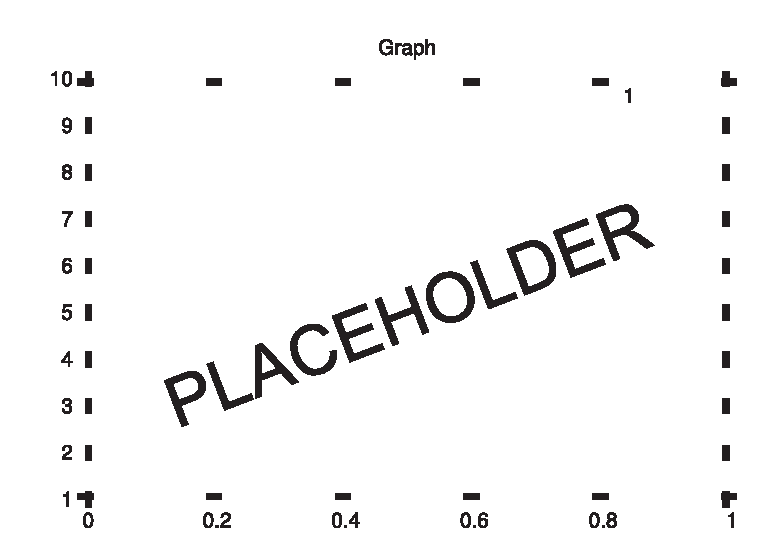
\includegraphics[width=\textwidth]{images/placeholder}
\end{figure}
}

\renewcommand{\algorithmicrequire}{\textbf{Input:}}
\renewcommand{\algorithmicensure}{\textbf{Output:}}
\renewcommand{\algorithmicforall}{\textbf{for each}}
\renewcommand{\algorithmiccomment}[1]{\textit{// #1}}

\renewcommand{\nomname}{List of Abbreviations}
\makenomenclature

\theoremstyle{definition}
\newtheorem{define}{Definition}[chapter]

\setlength{\hoffset}{-1in} %left margin will be 0, as hoffset is by default 1inch
\setlength{\voffset}{-1in} %analogous voffset
\setlength{\oddsidemargin}{4cm}
\setlength{\evensidemargin}{4cm}
\setlength{\topmargin}{25mm}
\setlength{\footskip}{1cm}
\setlength{\headheight}{0cm}
\setlength{\headsep}{0cm}
\setlength{\marginparwidth}{0cm}
\setlength{\marginparpush}{0cm}
\setlength{\textheight}{23.7cm}
\setlength{\textwidth}{14.5cm}
\let\openright=\clearpage

\def\mfauthor{Matej Vitásek}
\def\mfadvisor{RNDr. Irena Mlýnková Ph.D.}
\def\mfplacedate{Praha, 2011}

% Tato makra přesvědčují mírně ošklivým trikem LaTeX, aby hlavičky kapitol
% sázel příčetněji a nevynechával nad nimi spoustu místa. Směle ignorujte.
\makeatletter
\def\@makechapterhead#1{
  {\parindent \z@ \raggedright \normalfont
   \Huge\bfseries \thechapter. #1
   \par\nobreak
   \vskip 20\p@
}}
\def\@makeschapterhead#1{
  {\parindent \z@ \raggedright \normalfont
   \Huge\bfseries #1
   \par\nobreak
   \vskip 20\p@
}}
\makeatother

\def\chapwithtoc#1{
\chapter*{#1}
\addcontentsline{toc}{chapter}{#1}
}

\begin{document}

\lefthyphenmin=2
\righthyphenmin=2

%%% Titulní strana práce ======================================================
\pagestyle{empty}
\begin{center}

\large

Charles University in Prague

\medskip

Faculty of Mathematics and Physics

\vfill

{\bf\Large MASTER THESIS}

\vfill

\centerline{\mbox{
\includegraphics[width=60mm]{logo}}}

\vfill
\vspace{5mm}

{\LARGE \mfauthor}

\vspace{15mm}

% exactly as assigned
{\LARGE\bfseries Inference of XML Integrity Constraints}

\vfill

% Název katedry nebo ústavu, kde byla práce oficiálně zadána
% (dle Organizační struktury MFF UK)
Department of Software Engineering

\vfill

\begin{tabular}{rl}

Supervisor of the master thesis: & 	\mfadvisor \\
\noalign{\vspace{2mm}}
Study programme: & Informatika \\
\noalign{\vspace{2mm}}
Specialization: & ISS \\
\end{tabular}

\vfill

% Zde doplňte rok
\mfplacedate 

\end{center}



\newpage % ============================================================
%%% Následuje vevázaný list -- kopie podepsaného "Zadání diplomové práce".
%%% Toto zadání NENÍ součástí elektronické verze práce, nescanovat.
\openright

\noindent
[Sample: Here you may thank whoever you wish (the supervisor of the thesis, the consultant,
the person who lent the software, literature, etc.)]

TODO thank jInfer team, Mlynkova, anyone helping create this, colleagues at work...


\newpage % ============================================================
%%% Strana s čestným prohlášením k diplomové práci
\vglue 0pt plus 1fill
\noindent
I declare that I carried out this master thesis independently, and only with the cited
sources, literature and other professional sources.

\medskip\noindent
I understand that my work relates to the rights and obligations under the Act No.
121/2000 Coll., the Copyright Act, as amended, in particular the fact that the Charles
University in Prague has the right to conclude a license agreement on the use of this
work as a school work pursuant to Section 60 paragraph 1 of the Copyright Act.

\vspace{10mm}

\hbox{\hbox to 0.5\hsize{%
In ........ date ............
\hss}\hbox to 0.5\hsize{%
signature
\hss}}

\vspace{20mm}



\newpage % ============================================================
%%% Povinná informační strana diplomové práce
\vbox to 0.5\vsize{
\setlength\parindent{0mm}
\setlength\parskip{5mm}

Název práce: Odvozování integritních omezení v XML % TODO how to translate this correctly?

Autor: \mfauthor

Katedra:  Katedra softwarového inženýrství

Vedoucí diplomové práce: \mfadvisor{}, Katedra softwarového inženýrství

Abstrakt: [abstract of 80-200 words in Czech, but not a copy of the assignment of the
master thesis]

Klíčová slova:  XML, ID atributy, odvozování

\vss}\nobreak\vbox to 0.49\vsize{
\setlength\parindent{0mm}
\setlength\parskip{5mm}

Title:  Inference of XML Integrity Constraints

Author: \mfauthor

Department: Department of Software Engineering

Supervisor: \mfadvisor{}, Department of Software Engineering

Abstract:  [abstract of 80-200 words in English, but not a copy of the assignment of
the master thesis]

Keywords: XML, ID attributes, inference

\vss}

\newpage

%%% Strana s automaticky generovaným obsahem diplomové práce. U matematických
%%% prací je přípustné, aby seznam tabulek a zkratek, existují-li, byl umístěn
%%% na začátku práce, místo na jejím konci.

\openright
\pagestyle{plain}
\setcounter{page}{1}
\tableofcontents

% =============== TEXT ================
\newpage

% TODO what style of quotation marks to use? 
% TODO how to format text? is textit / texttt / ... OK?

\chapwithtoc{Preface}

Along with technologies like JSON, SQL/noSQL databases and bla, XML is one of the leading formats for storing structured data. However, even though languages such as DTD and XML Schema to describe XML structure already exist since a long time, most of the documents use outdated or no schema at all (link Vosta's Even ant can create...). To tackle this problem one may employ reverse-engineering techniques to infer the schema from existing documents, such as those described in A, B, C, jInfer. But the schema is not the only constraint that can be imposed on an XML document: the concept of \textit{keys} and \textit{foreign keys}, well known from the relational database world, applies here as well. One could go even further and try to find even more sophisticated relations in the data, such as \textit{functional dependencies} (link Sviro).

This work will be building upon the achievements of jInfer schema inference framework (TODO link Anti's improvements in schema inference), expanding its possibilities in the field of search for \textit{key-} and \textit{foreign key-}like structures in existing XML documents.

TODO Integrity constraints can be keys (with ID attributes as a "sub-group"), FKs, functional dependencies (quote Sviro), etc.
We will focus on the first kind - ID and IDREF attributes.

TODO argument: test data with DTD (and thus possibly ID/IDREF) is more common, we can have better test sets.

\section{Structure of the thesis}

The thesis will be structured as follows. 

First, we will introduce a few notions required throughout the work, such as XML tree, ID attributes, ID sets and keys for XML. 

Secondly, we will review approaches to ID attribute and XML keys search from previous articles on this topic. 

This will lead us to the NP-complete problem of maximal independent set (IS)\nomenclature{IS}{Independent Set}, where we will inspect approaches for solving it.

We will discuss a closely related Mixed Integer Problem (MIP)\nomenclature{MIP}{Mixed Integer Problem} and prove their "equality".

Afterwards, we will show how to use an external MIP solver and various heuristics to tackle this problem.

An extension to jInfer for finding ID attributes using MIP solver and a combination of heuristics will be presented and experimentally evaluated in the closing chapters.

\section{Conventions}

TODO list conventions - how we write code related stuff, module names, heu names, etc

\chapter{Definitions}
\label{chapter-definitions}

\section{XML Tree}

We shall use the representation introduced in \cite{fidax}, where an XML file is represented by a labeled tree consisting of nodes for elements, attributes and simple text data. Parent nodes are connected to child nodes with edges. This tree shall be called an \textit{XML tree}. For a given node $v$ of an XML tree we define $label(v)$ (name of the node in in the document, only for elements and attributes), $id(v)$ (unique identifier across the document) and $value(v)$ (text content, only for attributes and simple text data) in the same way as the cited article does.

Without loss of generality we ignore the actual ordering of nodes in the tree.

\paragraph{Example}

This example introduces an XML file fragment that will be used for demonstration throughout this work. An XML tree representing it is in Figure \ref{image-definitions-example-xml-tree}(a), where each node is annotated with a triplet $label(v) : id(v) : value(v)$.

\begin{verbatim}
<x>
  <y a="1" b="2"/>
  <y a="3" c="4"/>
  <y/>
  <z a="1"/>
</x>
\end{verbatim}

\begin{figure}
  \caption{Example XML Tree}
  \label{image-definitions-example-xml-tree} 
  \centering
    \subfigure[XML tree]{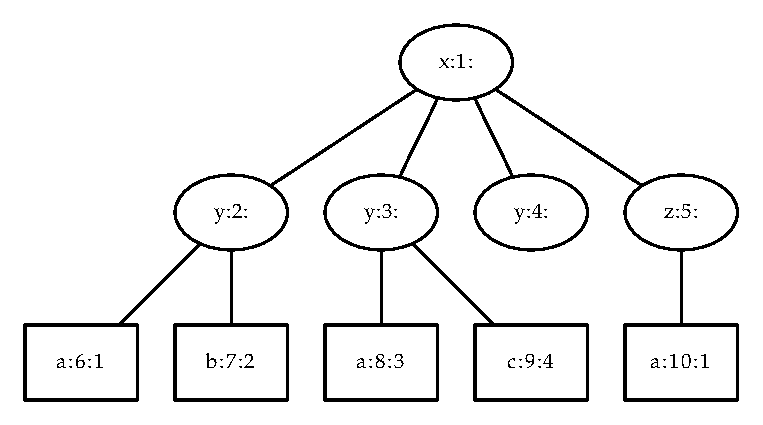
\includegraphics[width=.45\textwidth]{images/definitions/xml-tree}}
    \subfigure[Attribute Mappings]{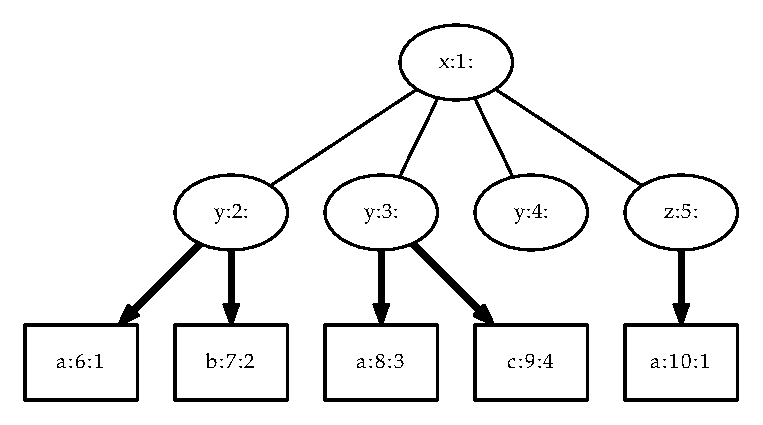
\includegraphics[width=.45\textwidth]{images/definitions/xml-tree-ams}}
\end{figure}

Furthermore, we denote $\mathcal{I}$ the set of all ids and $\mathcal{V}$ the set of all values in the document. We will need two more definitions from the article.

\begin{define}[Node equality]
	Nodes $v_1$ and $v_2$ are \textit{node equal}, written $v_1 =_n v_2$ iff $id(v_1) = id(v_2)$.
\end{define}

\begin{define}[Value equality]
	Nodes $v_1$ and $v_2$ are \textit{value equal}, written $v_1 =_v v_2$ iff $value(v_1) = value(v_2)$.
\end{define}

\section{\texttt{ID}, \texttt{IDREF}, \texttt{IDREFS} Attributes}
\label{section-definitions-id-attributes}

According to \cite{Bray:08:EML}, an XML attribute may have the type \texttt{ID}, \texttt{IDREF} or \texttt{IDREFS} (among others). The following constraints are related to these types.

\begin{quote}
\textbf{Validity constraint: \texttt{ID}}

Values of type \texttt{ID} \textsc{must} match the Name production. A name \textsc{must not} appear more than once in an XML document as a value of this type; i.e., \texttt{ID} values \textsc{must} uniquely identify the elements which bear them.

\textbf{Validity constraint: One \texttt{ID} per Element Type}

An element type \textsc{must not} have more than one \texttt{ID} attribute specified.

\textbf{Validity constraint: \texttt{ID} Attribute Default}

An \texttt{ID} attribute \textsc{must} have a declared default of \texttt{\#IMPLIED}\footnote{\texttt{\#IMPLIED} means that the attribute has a specified default value.} or \texttt{\#REQUIRED}\footnote{\texttt{\#REQUIRED} means that the attribute cannot be empty.}.

\textbf{Validity constraint: \texttt{IDREF}}

Values of type \texttt{IDREF} \textsc{must} match the Name production, and values of type \texttt{IDREFS} \textsc{must} match Names; each Name \textsc{must} match the value of an \texttt{ID} attribute on some element in the XML document; i.e. \texttt{IDREF} values \textsc{must} match the value of some \texttt{ID} attribute.
\end{quote}

\section{Attribute Mappings}
\label{section-definitions-ams}

Now we return to \cite{fidax} to define the notion of an \textit{attribute mapping} (or AM for short). \nomenclature{AM}{Attribute Mapping}
We will use a different definition (without introducing keys from \cite{keX}) that will however give us the same result.

\begin{define}[$\Sigma^E$, $\Sigma^A$, $\Sigma$]
	$\Sigma^E$ is the set of all element labels, $\Sigma^A$ is the set of all attribute labels. $\Sigma = \Sigma^E \cup \Sigma^A$ is their union and effectively the set of all labels in the document.
\end{define}

\begin{define}[Attribute mapping]
	For $x \in \Sigma^E$ and $y \in \Sigma^A$ we define the \textit{attribute mapping} of y over x, denoted $M_{x}^{y}$, the $\mathcal{I} \times \mathcal{I}$ relation defined by
	\[M_{x}^{y} = \{ (z,w): label(z) = x, label(w) = y, parent(w) = z \}.\]
\end{define}

Thus the relation $M_{x}^{y}$ contains edges in the XML tree connecting element nodes labeled $x$ and attribute nodes labeled $y$.

We can use projection to retrieve all the unique \textit{ids} of either elements or attributes from the relation, with notation $\pi_E(M_{x}^{y})$ and $\pi_A(M_{x}^{y})$.

\begin{define}[Type of the attribute mapping]
	Attribute mapping $M_{x}^{y}$ is of the \textit{type} $\tau(M_{x}^{y}) = x$.
\end{define}

\paragraph{Example}
The XML tree from Figure \ref{image-definitions-example-xml-tree}(b) has the following non-empty AMs drawn in bold lines: $M_{y}^{a} = \{(2,6), (3,8)\}$, $M_{y}^{b} = \{(2,7)\}$, $M_{y}^{c} = \{(3,9)\}$ and $M_{z}^{a} = \{(5,10)\}$.

The following example equations hold.
\begin{eqnarray*}
\pi_E(M_{y}^{a}) & = & \{2, 3\} \\
\pi_A(M_{z}^{a}) & = & \{10\} \\
\tau(M_{y}^{c}) & = & y
\end{eqnarray*}

\begin{define}[Image of the attribute mapping]
	\textit{Image} $\iota$ of the attribute mapping $M_{x}^{y}$ is defined as $\iota(M_{x}^{y}) = \{z: z = value(w), w \in \pi_A(M_{x}^{y})\}$.
\end{define}

So the image of an AM is a set of all the values of all the attribute nodes contained in the mapping.

\paragraph{Example}
Again referring to the XML tree from Figure \ref{image-definitions-example-xml-tree}, we get the following AM images.
\begin{eqnarray*}
\iota(M_{y}^{a}) & = & \{1, 3\} \\
\iota(M_{y}^{b}) & = & \{2\} \\
\iota(M_{y}^{c}) & = & \{4\} \\
\iota(M_{z}^{a}) & = & \{1\} \\
\end{eqnarray*}

\paragraph{Attribute Mapping Model}
An attribute mapping model is a data structure containing the information about all the AMs in a document, together with their images. We shall use this notion later in experimental part of this work.

\begin{define}[$name()$]
	Given an attribute mapping $m = M_{x}^{y}$, $name(m)$ shall be defined as the string $x-y$.
\end{define}

\section{ID Set}
\label{section-definitions-id-set}

Based on the requirements for an \texttt{ID} attribute from Section \ref{section-definitions-id-attributes} we will define ID set with the help of the following definition.

\begin{define}[Candidate attribute mapping]
An attribute mapping $m$ is a~\textit{candidate attribute mapping} if it is an injective function, that is,
\[|m| = |\pi_E(m)| = |\pi_A(m)| = |\iota(m)|.\]
\end{define}

\paragraph{Example}
In our example all the attribute mappings are candidate AMs.

Now we can proceed to define an ID set.

\begin{define}[ID set]
A set of candidate attribute mappings $I = \{m_1, \ldots m_n\}$ is an \textit{ID set} iff
\[\bigcap_{m_i \in I} \tau(m_i) = \emptyset \wedge \bigcap_{m_i \in I} \iota(m_i) = \emptyset.\]
\end{define}

That is, an ID set has images without repeating values and all the types are unique (an element cannot have more than one \texttt{ID} attribute).

\paragraph{Example}
Returning to our example, the following are all the possible ID sets: $\{ M_{y}^{a} \}, \{ M_{y}^{b} \}, \{ M_{y}^{b}, M_{z}^{a} \}, \{ M_{y}^{c} \}, \{ M_{y}^{c}, M_{z}^{a} \}$. Note that once we select an AM of type $y$ we can never add any other with the same type. Note also that $\{ M_{y}^{c}, M_{z}^{a} \}$ is not an ID set, because $\iota(M_{y}^{c}) \cap \iota(M_{z}^{a}) \neq \emptyset$.

\subsection*{\texttt{IDREF} and \texttt{IDREFS} Condition}

Given an ID set $I$, the requirements from Section \ref{section-definitions-id-attributes} give us the following condition for an attribute mapping $m$ to be marked \texttt{IDREF}:
\[\iota(m) \subseteq \bigcup_{m_i \in I} \iota(m_i).\]
Furthermore, if $m$ contains multivalued attributes, it is to be marked \texttt{IDREFS}.

\section{Attribute Mapping Weight}
\label{section-definitions-weight}

This definition of weight for AMs or AM sets comes from \cite{fidax} again. Let $M = \{m_1, \dots m_i\}$ be the set of all non-empty AMs in the document.

\subsection{Support}

\begin{define}[Support]
\textit{Support} of an attribute mapping $m$ is defined as follows:
\[\phi(m) = \frac{|m|}{\sum_{p \in M}|p|}.\]
\end{define}

\begin{quote}
The support of attribute mapping $M_x^y$ is the fraction of edges in~the~XML tree that connect $x$ elements to $y$ attributes.
\end{quote}

\paragraph{Example}
Support of $M_{y}^{a}$ in our example is $2 / (2+1+1+1) = 0.4$. Support of~every other mapping is $1 / (2+1+1+1) = 0.2$.\\

\subsection{Coverage}

\begin{define}[Coverage]
\textit{Coverage} of an attribute mapping $m$ is defined as follows:
\[\chi(m) = \left( \sum_{p \in M, p \neq m} |\iota(m) \cap \iota(p)| \right) / \sum_{p \in M} |\iota(p)|.\]
\end{define}

\begin{quote}
The coverage of an attribute mapping measures how much of the image of that mapping occurs elsewhere, as a fraction of all mappings images in the document.
\end{quote}

\paragraph{Example}
Coverage of $M_{y}^{a}$ in our example is $(0+0+1) / (2+1+1+1) = 0.2$. Coverage of $M_{z}^{a}$ is $0.2$ as well, all the other mappings have coverage $0$.
\\

\textit{Weight} of an attribute mapping is then defined as a linear combination of its support and coverage.

\begin{define}[Weight]
For $\alpha, \beta \geq 0$ as relative priorities of support and coverage we define the AM \textit{weight} as follows:
\[weight(m) = \alpha . \phi(m) + \beta . \chi(m).\]
For a set of AMs (which may or may not be an ID set) $S = \{m_1, \ldots m_i\}$ we define the weight of this set as the sum of the weights of its AMs:
\[weight(S) = \sum_{m \in S} weight(m).\]
\end{define}

Note that this definition of weight is quite arbitrary and all the algorithms mentioned later could easily work with AM weight defined in any other way, even for example defined interactively by the user.

\section{Independent Set}
\label{section-definitions-is}

\nomenclature{IS}{Independent Set}

We shall need the notion of an indepentent set (IS) of vertices in a graph and its weighted variant.

\begin{define}[Independent set]
Given an undirected graph $G = (V, E)$, a set of vertices $I \subseteq V$ is an \textit{independent set}, iff
\[\forall v_1, v_2 \in I, v_1 \neq v_2: (v_1, v_2) \notin E.\]
\end{define}

\begin{define}[Maximum weighted independent set]
Given an undirected graph $G = (V, E)$ and a weight function $w: V \rightarrow \mathbb{R}$, an independent set $I_{max}$ is the \textit{maximum weighted independent set}, iff the following is satisfied:
\[\forall I' \subseteq V, I' \text{is an independent set}: \sum_{v \in I'} w(v) \leqslant \sum_{v \in I_{max}} w(v).\]
\end{define}

It is well known that finding the maximum weighted IS is an NP-hard optimization problem, \cite{JM1986425}.

\section{Linear Programming}

The problem of \textit{linear programming} is optimization of a~linear function under a~set of linear constraints. The formulation is usually called a~\textit{linear program}. 

It can be written in the following form:

\begin{eqnarray*}
\max_{x} z & = & \mathbf{c}^{\mathrm{T}}\mathbf{x} \\
s.t.\, A\mathbf{x} & \leqslant & \mathbf{b} \\
\mathbf{x} & \geqslant & 0 \\
\end{eqnarray*}
\[
\mathbf{x} =
\begin{bmatrix}
x_1 \\
x_2 \\
\ldots \\
x_n \\
\end{bmatrix},
\mathbf{c} = 
\begin{bmatrix}
c_1 \\
c_2 \\
\ldots \\
c_n \\
\end{bmatrix},
\mathbf{b} =
\begin{bmatrix}
b_1 \\
b_2 \\
\ldots \\
b_m \\
\end{bmatrix},
\]

where a minimization version is possible, too.

Where $\mathbf{x}$ is the vector of variables (to be found by the optimization), $\mathbf{b}$ is the vector and $A$ its accompanying matrix of constraints and $\mathbf{c}$ is the vector of coefficients for the objective function. $\mathbf{x}$ and $\mathbf{c}$ have length $n$, $\mathbf{b}$ has length $m$ and $A$ has dimensions $m \times n$. Furthermore, \[\max_{x} f(x)\] means maximize the value of $f(x)$ by changing the value of $x$.\\

Another way to write this formulation is this:

\begin{eqnarray*}
\max_{x} z = \sum_{i=1}^{n} c_i x_i \\
s.t. & \\
	   a_{11}x_{1} + a_{12}x_{2} + \ldots + a_{1n}x_{n} & \leqslant & b_{1} \\
	   a_{21}x_{1} + a_{22}x_{2} + \ldots + a_{2n}x_{n} & \leqslant & b_{2} \\
	   \ldots \\
	   a_{m1}x_{1} + a_{m2}x_{2} + \ldots + a_{mn}x_{n} & \leqslant & b_{m} \\
	   x_i \geqslant 0, i = 1, \ldots n \\
\end{eqnarray*}

Solving a linear program is usually possible in polynomial time using the~\textit{simplex algorithm} described for example in \cite{dantzig1998linear}.

\section{Mixed Integer Problem}

\nomenclature{MIP}{Mixed Integer Problem}

\begin{define}[Mixed integer problem]
	MIP, or \textit{mixed integer problem}, is an~instance of~linear programming in~which some or~all variables are limited to~integral or~boolean (0, 1) values.
\end{define}

Solving MIP in general is $\NP$-hard.

\chapter{Related Work}
\label{chapter-research}

According to the article \cite[Chapter~4]{fidax}, the problem of finding an ID set with weight more than some $K$ ($K$-\textsc{IDSet}) is in NP. Furthermore, the independent set (IS) problem can be reduced to $K$-\textsc{IDSet}, meaning $K$-\textsc{IDSet} is NP-hard and thus NP-complete. The transformation from IS problem formulation to~$K$-\textsc{IDSet} problem formulation is as follows.

\begin{quote}
Let $G = (V, E)$ be a simple connected graph with vertex set $V = \{v_1, \ldots, v_n\}$, and edge set $E = \{e_1, \ldots, e_m\}$. We define the attribute mappings as follows. Let $ \mathcal{I} = V \cup E$, and define $value(x) = x, x \in \mathcal{I}$. For each vertex $v_i \in V$, we create a mapping $m_i = \{(v_i, e_j): e_j \in E \,\text{is incident on}\, v_i \}$, and define $\tau(m_i) = v_i$; let $C = \{m_1, \ldots, m_n\}$ be set of all such mappings. It is clear that G has an independent set of size $K$ iff $C$ has an ID set of size $K$. Also, $C$ can be constructed in time polynomial on $n+m$.
\end{quote}

The article continues by proving that finding the maximum weighted IS can be reduced to the problem of finding an ID set with maximum weight (\textsc{Max-IDSet}). This again means that \textsc{Max-IDSet} is NP-complete and, furthermore, unless $\P = \NP$, \textsc{Max-IDSet} has no constant factor approximation algorithm.

The difference in transformation from maximum weighted IS to \textsc{Max-IDSet} is as follows.

\begin{quote}
[...] with the added restriction that $w(m_i) = w(v_i), v_i \in V$.
\end{quote}

Note that the transformation works in both ways: it is equivalently possible to create a maximum weighted IS instance for a given \textsc{Max-IDSet} instance.

The article further suggests a heuristic approach described in Section \ref{section-mip-fidax}, which was incorporated into the framework proposed by this work.

To the best of our knowledge, there are no other articles dealing with this problem.\\

\section{Finding XML Keys}

XML keys are a structure somewhat similar to \texttt{ID} attributes, but with a much larger expressive strength. They have been introduced in \cite{keX} and implemented in XML Schema\footnote{\url{http://www.w3.org/TR/xmlschema11-1/\#Identity-constraint\_Definition\_details}}.

Fajt in \cite{fajt} summarizes several algorithms to help find XML keys in existing data, namely \textit{Gordian}, \textit{XML Primary Keys}, \textit{SPIDER} and \textit{DBA Companion}. Except for \textit{XML Primary Keys}, they all are originally purposed to find keys in~relational databases. We will describe them shortly.

\subsubsection{\textit{Gordian}}

This algorithm from \cite{fajt-41} extracts composite primary keys (PKs) from relational databases.

\begin{quote}
The idea behind is an observation that a projection of entities corresponds to a key if each counted aggregation for a projection is equal to 1. Thus, this method searches for all possible projections of a dataset while computing aggregations on the projected part of the set of entities.
\end{quote}

This is achieved by constructing a prefix tree from the tuples in the original relation, which is then pruned and traversed depth-first to find non-key attributes from which the primary keys are inferred. This algorithm still has to~be~adapted to~search for PKs in XML data.

\subsubsection{\textit{XML Primary Keys}}

This is an algorithm from \cite{fajt-39} capable of finding simple keys and foreign keys directly in XML data. This is achieved by building a prefix tree containing all the XML nodes and then evaluating every path in it as a candidate key using metrics called \textit{support} and \textit{confidence}. To find more complex keys, the algorithm iteratively constructs candidate keys from simpler ones and evaluates them.\\

The following two algorithms deal with \textit{inclusion dependencies} (INDs), described for example in \cite{fajt-12}.

\subsubsection{\textit{SPIDER}}

The core of this algorithm from \cite{fajt-51, fajt-53} is the following.

\begin{quote}
The process consists of two steps - sets of values are sorted during the first one and then all the candidates are analyzed in parallel. The core of the method is utilizing the data structure called min-heap which synchronizes the processing of all values of all attributes.
\end{quote}

It is~possible to~use a~number of~heuristic pruning strategies to~keep the~min-heap in~a~reasonable size. This algorithm performs very well for PKs in~relational databases, however, it~still has to~be~adapted for~XML keys.

\subsubsection{\textit{DBA Companion}}

Like \textit{SPIDER}, this method from \cite{fajt-53} is able to find all the~INDs in~the~da\-ta\-base in~just one pass. However, it~uses a~different data structure (basically a~binary relation between the~attributes and~their corresponding values) and~considers data types. Composite INDs are~found using the~simple ones and~pruning the~search space. According to~the~authors of~\textit{SPIDER}, \textit{DBA Companion} is~far inferior in~performance. This algorithm has yet to~be~adapted to~search for XML keys, too.

\subsubsection{Fajt's Approach - \textit{KeyMiner}}

Fajt introduces a new algorithm based on \textit{Gordian} and \textit{SPIDER} to look for primary and foreign keys in XML data. First, relations have to be extracted from the original XML document. Then all the primary keys are found using a modified \textit{Gordian} algorithm which can find absolute as well as relative PKs. Finally, \textit{SPIDER} is used to compute the foreign keys from the PKs found in the previous step.

\subsection{Relation to \texttt{ID} Attributes}

XML keys found this or any other way can under some circumstances (when they are simple enough) be translated to an equivalent \texttt{ID} attribute definition. The process is described in \cite[Ch.\ 9, s.\ 3]{vlist2002xml}. This opens a new line of possible research: finding XML keys using an algorithm modified to look only for \textit{useful} keys and then converting them to \texttt{ID} attributes.\\ 

However, in our work we find \texttt{ID} attributes directly. And even though we can always convert them to XML keys by the process mentioned above, we are unable to find more complex keys this way.\\

\section{Maximum Weighted IS}

Maximum weigthed IS is a well researched topic with a lot of known direct or approximation algorithms, see e.g. \cite{JM1986425} or \cite{Fomin:2009:MCA:1552285.1552286}. According to for example \cite{Paschos:1997:SAO:254180.254190}, the best known approximation algorithm for weighted IS to-date achieves an approximation ratio of $3(\Delta + 2)$, where $\Delta$ is the maximum degree of a vertex in the IS graph. This article lists several algorithms similar to those we introduce in the following chapters.\\

\chapter{MIP Approach}
\label{chapter-mip}

In this chapter we introduce a new approach to finding maximum ID sets. First, we transform the problem formulation to maximum weighted IS problem formulation. Then we transform this into a MIP formulation, and demonstrate how this can be solved using a solver such as GLPK. \nomenclature{GLPK}{GNU Linear Programming Kit}
We will continue by applying heuristical approaches to improve the performance of the process.

\section{ID Set to IS Formulation}

Given $C = \{m_1, \ldots, m_n\}$ a set of all AMs in a document, we construct a graph $G = (V,E)$ as follows. For each AM $m_i \in C$ we create a vertex $v_{name(m_i)}$. Two vertices $v_{name(m_i)}$ and $v_{name(m_j)}$ shall be connected by an edge iff they cannot share the same ID set, either because they have the same type ($\tau(m_i) = \tau(m_j)$), or their images intersect ($\iota(m_i) \cap \iota(m_j) \neq \emptyset$). Weight of a vertex $v_{name(m_i)}$ is the weight of the attribute mapping: $w(v_{name(m_i)}) = weight(m_i)$.

Now finding the maximum weighted IS in $G$ finds the maximum (optimal) ID set in the original document.

\section{IS to MIP Formulation}

Given a graph $G = (V,E)$ with a weight function $w: V \rightarrow \mathbb{R}$, we introduce a binary variable $x_i$ for each vertex $v_i \in V$ and an inequality constraint $x_i + x_j \leq 1$ for each edge $e = (v_i, v_j) \in E$. Furthermore we introduce an objective function in form $\sum_{x_i} x_i w(v_i)$.

It is obvious that the objective function and all the constraints consitute a MIP instance, and that solving it finds the maximum weigthed IS in $G$.

\section{Finding ID Sets With GLPK}

By chaining these two translations we can create a MIP formulation for a given set of AMs from a document. Solving this MIP instance will give us the optimal ID set for this document.

GLPK \cite{glpk} is a multi-platform, multi-purpose solver well suited for this task. It uses the Simplex method to solve LP problems and \textit{Branch \& Bound} (see \cite{land60a} for details) for MIP. An advantage of using \textit{Branch \& Bound} is that while traversing the \textit{search tree} it finds intermittent, sub-optimal solutions. It is thus possible to limit the total search time and instead of the optimum take the best solution found so far.\\

We will now demonstrate the full process of finding the optimal ID set of an example XML file using GLPK.

\subsection{Example}

Consider again our XML file fragment.

\begin{verbatim}
<x>
  <y a="1" b="2"/>
  <y a="3" c="4"/>
  <y/>
  <z a="1"/>
</x>
\end{verbatim}

Recall that attribute mappings in this example are $C = \{M_{y}^{a}, M_{y}^{b}, M_{y}^{c}, M_{z}^{a}\}$. Corresponding vertices in the IS formulation will be $V = \{v_{y-a}, v_{y-b}, v_{y-c}, v_{z-a}\}$. Edges in the IS formulation will be the following.

\begin{eqnarray*}
(v_{y-a},v_{y-b}) \\
(v_{y-a},v_{y-c}) \\
(v_{y-b},v_{y-c}) \\
(v_{y-a},v_{z-a}) \\
\end{eqnarray*}

First three edges are due to the type collision ($y$), the last one is due to $\iota(M_{y}^{a}) \cap \iota(M_{z}^{a}) = \{1\}$. The graph $G$ constructed in this way is in Figure \ref{image-mip-is-graph}.

\begin{figure}
  \caption{IS Representation Graph}
  \label{image-mip-is-graph}
  \centering
	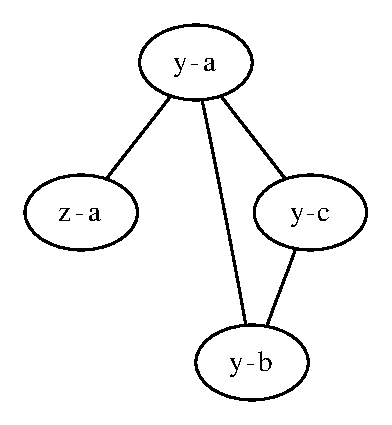
\includegraphics[width=.25\textwidth]{images/is-representation}
\end{figure}

The next step is the MIP formulation. We do not need to translate from the IS formulation, as the translation from ID set formulation is straightforward, too. For each AM $m$ there will be one binary variable $x_{name(m)}$. Objective function coefficients in vector $\mathbf{c}$ will be weights of respective mappings. For each pair of AMs $m_1, m_2$ that cannot share the same ID set there shall be a row in matrix $A$ representing the inequality $x_{name(m_1)} + x_{name(m_2)} \leqslant 1$. $\mathbf{b}$ will be a vector of ones with corresponding length.

\[
\mathbf{x} =
\begin{bmatrix}
x_{y-a} \\
x_{y-b} \\
x_{y-c} \\
x_{z-a} \\
\end{bmatrix},
\mathbf{c} = 
\begin{bmatrix}
weight(M_{y}^{a}) \\
weight(M_{y}^{b}) \\
weight(M_{y}^{c}) \\
weight(M_{z}^{a}) \\
\end{bmatrix} =
\begin{bmatrix}
0.2 \\
0.2 \\
0.6 \\
0.4 \\
\end{bmatrix},
\mathbf{b} =
\begin{bmatrix}
1 \\
1 \\
1 \\
1 \\
\end{bmatrix},
A =
\begin{pmatrix}
0 & 1 & 1 & 0 \\
1 & 0 & 1 & 0 \\
1 & 1 & 0 & 0 \\
1 & 0 & 0 & 1 \\
\end{pmatrix}
\]

The problem now is, recall, to solve the following.

\begin{eqnarray*}
\max_{x} z & = & \mathbf{c}^{\mathrm{T}}\mathbf{x} \\
s.t.\, A\mathbf{x} & \leqslant & \mathbf{b} \\
\end{eqnarray*}

In GLPK \textit{MathProg} language, this translates to the following formulation. % TODO cite mathprog

\begin{scriptsize}
\begin{verbatim}
set AMs;
param Weight {i in AMs};
var x {i in AMs} binary;
maximize z: sum {i in AMs} x[i] * Weight[i];
s.t. c1: x['y-a'] + x['y-b'] <= 1;
s.t. c2: x['y-a'] + x['y-c'] <= 1;
s.t. c3: x['y-b'] + x['y-c'] <= 1;
s.t. c4: x['y-a'] + x['z-a'] <= 1;
data;
set AMs := y-a y-b y-c z-a;
param Weight :=
y-a 0.6
y-b 0.2
y-c 0.2
z-a 0.4;
end;
\end{verbatim}
\end{scriptsize}

We can use this as an input for the GLPK solver, and we get the solution.

\begin{scriptsize}
\begin{verbatim}
...
Problem:    glpk_input
Rows:       5
Columns:    4 (4 integer, 4 binary)
Non-zeros:  12
Status:     INTEGER OPTIMAL
Objective:  z = 0.6 (MAXimum)

...

   No. Column name       Activity     Lower bound   Upper bound
------ ------------    ------------- ------------- -------------
     1 x[y-a]       *              1             0             1 
     2 x[y-b]       *              0             0             1 
     3 x[y-c]       *              0             0             1 
     4 x[z-a]       *              0             0             1 

...
\end{verbatim}
\end{scriptsize}

This output tells us that the solution is $x_{y-a} = 1$, $x_{y-b} = 0$, $x_{y-c} = 0$ and $x_{z-a} = 0$. This means that the optimal ID set with maximum weight contains only the $M_{y}^{a}$ attribute mapping.\\

It is obvious that this approach works and for any possible input we can let GLPK find the optimal solution. However, sometimes it takes too long to find the optimum (see e.g. Section \ref{section-glpk-comparison}), we should try to improve this process.

\section{Heuristics}

TODO what is heuristics (link wise books), what is metaheuristics (we will be using them)

TODO mention things like Taboo search and Genetic Algorithms (we can emulate them with Crossover/Mutation) (we won't be using them)

TODO we will be working with heuristics striving to do the following: input is a list of AMs, they have their weight, we try to find a non-conflicting subset which maximizes the weight

TODO we will be using a pool - what is a pool

\begin{figure}
  \caption{Metaheuristic schema}
  \label{image-metaheuristic}
  \centering
    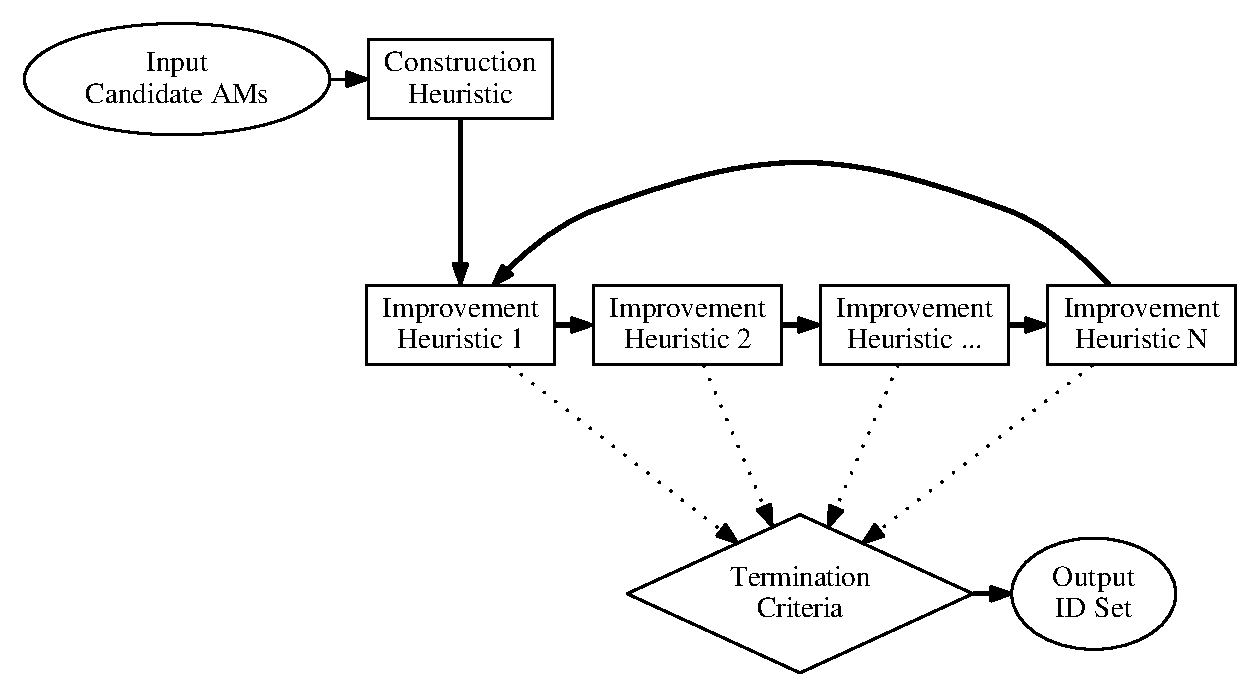
\includegraphics[width=\textwidth]{images/metaheuristic}
\end{figure}

\subsection{Constructions Heuristics}
% TODO can I format things in nomenclature?
\nomenclature{CH}{Construction Heuristic} %TODO decide on how to format CH/IH

TODO construction heuristics are heus that provide us with at least some solution.

\subsubsection{\heu{FIDAX}}
\label{section-mip-fidax}

It should be obvious by now that the algorithm described in \cite{fidax} (we shall call it \heu{FIDAX} from now on) can trivially be used as a construction heuristic that will give us one feasible solution.

The pseudocode of this CH (taken from the original article with trivial modifications without changing the logic) is in Listing \ref{listing-ch-fidax}.

\begin{algorithm}
\caption{\heu{FIDAX} CH}
\label{listing-ch-fidax}
\begin{algorithmic}
\REQUIRE $C$ list of candidate AMs
\ENSURE a feasible solution
\STATE $C' \gets C$ sorted by decreasing size
\STATE Compute the weight $w(m)$ of each $m$ in $C$
\FORALL{$t$ in $\Sigma^E$}
  \STATE Let $m$ be a \textbf{highest-weight} mapping of type $t$ in $C'$
  \STATE Remove from $C'$ all mappings of type $t$ except $m$
\ENDFOR
\FORALL{$m$ in $C'$}
  \STATE $S \gets$ all mappings in $C$ whose images intersect $\iota(m)$
  \IF{$w(m) > \sum_{p \in S} w(p)$}
    \STATE remove all $p \in S$ from $C'$
  \ELSE
    \STATE remove $m$ from $C'$
  \ENDIF
\ENDFOR
\RETURN $C'$
\end{algorithmic}
\end{algorithm}

\subsubsection{\heu{Random}}
\label{heu-ch-random}

One of the most natural heuristics when dealing with the IS problem can be described as follows: select from candidate AMs at random, if possible (addition would not violate the ID set condition) add them to the solution. This is obviously a hungry heuristic. %TODO have I defined ID set condition yet??

The advantages of this trivial heuristic are simplicity, speed and ease with which it can create a pool of variable solutions, almost for free. As we will see later in the experiments (Section \ref{section-experiments-random-fuzzy-fidax}), it performs surprisingly well.

See the Listing \ref{listing-ch-random} for its pseudocode.

\begin{algorithm}
\caption{\heu{Random} CH}
\label{listing-ch-random}
\begin{algorithmic}
\REQUIRE $N$ required size of pool
\REQUIRE $C$ list of candidate AMs
\ENSURE pool of $N$ feasible solutions
\STATE $r \gets $ empty pool
\FOR{$i = 1 \to N$}
  \STATE \COMMENT{create 1 solution}
  \STATE $s \gets $ empty solution
  \WHILE{$s$ is a feasible ID set}
    \STATE $a \gets $ pick at random from $C \backslash S$
    \STATE $s \gets s \cup a$
  \ENDWHILE
  \STATE $r \gets r \cup s$
\ENDFOR
\RETURN $r$
\end{algorithmic}
\end{algorithm}

\subsubsection{\heu{Fuzzy}}
\label{heu-ch-fuzzy}

\heu{Fuzzy} is an improvement over the \heu{Random} CH: it picks the next AM to try to add based on \textit{weighted} instead of uniform random. The weight used here is the usual weight of an AM as defined in TODO. Because of the randomness involved in the choice, we can again easily create a pool of solutions this way.

Again, this is a hungry heuristic, the Listing \ref{listing-ch-fuzzy} contains its pseudocode.

% TODO od I need to specify which are my own idea? I guess so, I should link any heu that is not mine. But do I need to stress that for example Fuzzy is mine?

\begin{algorithm}
\caption{\heu{Fuzzy} CH}
\label{listing-ch-fuzzy}
\begin{algorithmic}
\REQUIRE $N$ required size of pool
\REQUIRE $C$ list of candidate AMs
\ENSURE pool of $N$ feasible solutions
\STATE $r \gets $ empty pool
\FOR{$i = 1 \to N$}
  \STATE \COMMENT{create 1 solution}
  \STATE $s \gets $ empty solution
  \STATE $C' \gets C$

  \WHILE{$C' $ not empty}
    \STATE $a \gets $ pick at weighted random from $C'$
    \IF{$s \cup a$ is a feasible ID set}
      \STATE $s \gets s \cup a$
      \STATE $C' \gets C' \backslash a$
    \ENDIF
    \FORALL{$c \in C'$}
      \IF{$s \cup c $ is \textbf{not} a feasible ID set}
        \STATE \COMMENT {if $c$ cannot be possibly added anymore}
        \STATE $C' \gets C' \backslash c$
      \ENDIF
    \ENDFOR
  \ENDWHILE

  \STATE $r \gets r + s$
\ENDFOR
\RETURN $r$
\end{algorithmic}
\end{algorithm}

\subsubsection{\heu{Incremental}}

This trivial heuristics sorts all candidate AMs by their decreasing weights (Section \ref{section-definitions-weight}) and then tries to iteratively add them to solution, if possible. This way it can create only one solution, and again, this is a hungry heuristic.

See listing \ref{listing-ch-incremental}.

\begin{algorithm}
\caption{\heu{Incremental} CH}
\label{listing-ch-incremental}
\begin{algorithmic}
\REQUIRE $C$ list of candidate AMs
\ENSURE a feasible solution
\STATE $C' \gets $ sort $C$ by decreasing weight
\STATE $s \gets $ empty solution
\FORALL{$c \in C'$}
  \IF{$s \cup c$ is a feasible ID set}
    \STATE $s \gets s + c$
  \ENDIF
\ENDFOR
\RETURN $s$
\end{algorithmic}
\end{algorithm}

\subsubsection{\heu{Removal}}

This is basically a reversal of the idea from the \heu{Incremental} heuristic - start with a solution containing all the candidate AMs. This probably does not satisfy the ID set condition. Therefore, order them by increasing size and start removing them from the solution, until it satisfies the ID set condition. Again, this is a hungry heuristic returning only one solution.

See listing \ref{listing-ch-removal}.

\begin{algorithm}
\caption{\heu{Removal} CH}
\label{listing-ch-removal}
\begin{algorithmic}
\REQUIRE $C$ list of candidate AMs
\ENSURE a feasible solution
\STATE $C' \gets $ sort $C$ by increasing weight
\STATE $s \gets C'$
\FORALL{$c \in s$}
  \IF{$s$ is a feasible ID set}
    \RETURN $s$
  \ENDIF
  \STATE $s \gets s \backslash c$
\ENDFOR
\end{algorithmic}
\end{algorithm}

\subsubsection{Truncated Branch \& Bound}

This CH will be called \heu{Glpk} from now on, for it is basically a time-constrained run of GLPK.

TODO if we limit GLPK's runtime, we get this

TODO we shuffle AMs - we get different runs - pool is possible

\subsection{Improvement Heuristics}
\label{section-mip-ihs}

\nomenclature{IH}{Improvement Heuristic}

TODO what they are, that they need a pool sometimes, their input and output is a pool, ...

TODO mention intensification, diversification

TODO mention that combination of \heu{Crossover}, \heu{Mutation} and \heu{RemoveWorst} is a sort of genetic algorithm

\subsubsection{\heu{Identity}}

This ultimately trivial improvement heuristics does nothing. It simply returns the feasible pool unchanged. For the sake of completeness, see its listing \ref{listing-ih-identity}.

\begin{algorithm}
\caption{\heu{Identity} IH}
\label{listing-ih-identity}
\begin{algorithmic}
\REQUIRE $FP$ pool of feasible solutions
\ENSURE the same pool of feasible solutions
\RETURN $FP$
\end{algorithmic}
\end{algorithm}

\subsubsection{\heu{Remove Worst}}

This trivial IH tries to improve the solution pool by removing the worst solution (i.e. the one with the lowest quality). This might be interesting in cooperation with other improvement heuristics that increase the solution pool size, to keep it from growing by pruning inferior solutions.

See listing \ref{listing-ih-removeworst}.

\begin{algorithm}
\caption{\heu{Remove Worst} IH}
\label{listing-ih-removeworst}
\begin{algorithmic}
\REQUIRE $FP$ pool of feasible solutions
\ENSURE pool of feasible solutions
\STATE $s_{min} \gets $ solution with the lowest weight $\in FP$
\RETURN $FP \backslash s_{min}$
\end{algorithmic}
\end{algorithm}

\subsubsection{\heu{Random Remove}}

This is again a rather trivial IH, something which is usually referred to as a \textit{perturbation} function. % TODO link the notion
By removing a random subset of specified size from each solution in the pool, it provides variability needed to escape from local optima. % TODO make sure we have talked about local optima before

The number of AMs to remove from each solution is specified as ratio (from the interval $(0, 1)$) of the solution size. % TODO have we defined what a solution size is?
For example, \heu{Random Remove} with $ratio = 0.1$ would remove 1 random AM from a solution containing 10 AMs and 2 from a solution containing 17 AMs (due to rounding).

This heuristic returns a pool of solutions of the same size as it got on its input.

See listing \ref{listing-ih-randomremove}.

\begin{algorithm}
\caption{\heu{Random Remove} IH}
\label{listing-ih-randomremove}
\begin{algorithmic}
\REQUIRE $FP$ pool of feasible solutions
\REQUIRE $k \in (0,1)$ ratio of AMs to remove from each $s \in FP$
\ENSURE pool of feasible solutions
\FORALL{$s \in FP$}
  \STATE $K \gets k * |s|$
  \STATE remove $K$ random AMs from $s$
\ENDFOR
\RETURN $FP$
\end{algorithmic}
\end{algorithm}

\subsubsection{\heu{Hungry}}

This simple improvement heuristic assumes that the solutions in the pool are not ``complete", i.e. there are AMs that could be added to them without violating the ID set condition.

\heu{Hungry} tries to improve each solution in the feasible pool in the following way. It orders all candidate AMs not present in the solution by decreasing weight. Afterwards, it iteratively tries to extend the solution with these AMs, taking care not to violate the ID set condition. The resulting solution (whether any AMs were added or not) is then returned to the pool. Listing \ref{listing-ih-hungry} captures this process.

\begin{algorithm}
\caption{\heu{Hungry} IH}
\label{listing-ih-hungry}
\begin{algorithmic}
\REQUIRE $FP$ pool of feasible solutions
\REQUIRE $C$ list of candidate AMs
\ENSURE pool of feasible solutions
\FORALL{$s \in FP$}
  \STATE \COMMENT {improve a single solution}
  \STATE $C' \gets C \backslash s$
  \STATE $C' \gets C'$ sorted by decreasing weight
  \FORALL{$c \in C'$}
    \IF{$s \cup c$ is a feasible ID set}
      \STATE $s \gets s \cup c$
    \ENDIF
  \ENDFOR
\ENDFOR
\RETURN $FP$
\end{algorithmic}
\end{algorithm}

\subsubsection{\heu{Mutation}}

TODO explain how this works and link wise books

TODO explain how this translates to GLPK input

For every AM $AM_F$ fixed to appear in the solution a following constraint is added to GLPK input:
\[s.t. f_{index}: x['name(AM_F)'] = 1;\]
$index$ is a unique integer to number all the constraints.

Additionaly, every other mapping $AM_i$ colliding with $AM_F$ ($\iff \iota(AM_F) \cap \iota(AM_i) \neq \emptyset$) will cause the following constraint to be added:
\[s.t. f_{index}: x['name(AM_i)'] = 0;\]
And the original constraint in form:
\[s.t. c_{index}: x['name(AM_F)'] + x['name(AM_i)'] <= 1;\]
will not be included.

See listing \ref{listing-ih-mutation}.

\begin{algorithm}
\caption{\heu{Mutation} IH}
\label{listing-ih-mutation}
\begin{algorithmic}
\REQUIRE $FP$ pool of feasible solutions
\REQUIRE $k$ ratio of AMs to fix
\ENSURE pool of feasible solutions
\STATE $incumbent \gets $ best solution in $FP$ \COMMENT {best = highest weight}
\STATE $K \gets k * |incumbent|$
\STATE fix $K$ random AMs from $incumbent$ in GLPK problem formulation
\STATE $improved \gets $ run GLPK
\RETURN $FP \cup improved$
\end{algorithmic}
\end{algorithm}

\subsubsection{\heu{Crossover}}

TODO explain how this works and link wise books

TODO explain how this translates to GLPK input - it's again simple fixing to 1, but we get the list of AMs in a different manner.

See listing \ref{listing-ih-crossover}.

\begin{algorithm}
\caption{\heu{Crossover} IH}
\label{listing-ih-crossover}
\begin{algorithmic}
\REQUIRE $FP$ pool of feasible solutions
\REQUIRE $k$ ratio of solutions to look for commonalities in
\ENSURE pool of feasible solutions
\STATE $K \gets k * |FP|$
\STATE $FP' \gets K$ random solutions $\in FP$
\STATE $am \gets$ AMs found in all solutions $\in FP'$
\STATE fix $am$ in GLPK problem formulation
\STATE $improved \gets $ run GLPK
\RETURN $FP \cup improved$
\end{algorithmic}
\end{algorithm}

\subsubsection{\heu{Local Branching}}

TODO explain how this works and link wise books

TODO explain how this translates to GLPK input

A new constrain describing the maximal allowed distance from the incumbent solution is added to GLPK input.

\[s.t. LB: sum\{i\ in\ INCUMBENT\} (1 - x[i]) + sum\{i\ in\ REMAINING\} x[i] \leq k;\]

Where $INCUMBENT$ is a set of names of AMs in the incumbent solution, $REMAINING$ is a set of all the AMs not included in the incumbent solution and $k$ is the requested maximal distance.

See listing \ref{listing-ih-localbranching}.

\begin{algorithm}
\caption{\heu{Local Branching} IH}
\label{listing-ih-localbranching}
\begin{algorithmic}
\REQUIRE $FP$ pool of feasible solutions
\REQUIRE $k$ ratio of total AM count to bound the Hamming distance to
\ENSURE pool of feasible solutions
\STATE $K \gets k * |$total AM count$|$
\STATE $incumbent \gets $ best solution in $FP$ \COMMENT {best = highest weight}
\STATE add max Hamming distance requirement to GLPK problem formulation
\STATE $improved \gets $ run GLPK
\RETURN $FP \cup improved$
\end{algorithmic}
\end{algorithm}

\section{IDREF}

Once an ID set is found, regardless of how exactly, it is easy to find the IDREF set, i.e. the attribute mappings that can be declared as IDREF. % TODO link FIDAX, they did it first.

First of all, from the set of all the attribute mappings in the model remove all the AMs contained in the ID set. This is because the specification % TODO link to the specific anchor in the page
does not allow an attribute to be ID and IDREF (IDREFS) at the same time. Let us denominate these mappings as \textit{IDREF candidates} (obviously different from \textit{candidate AMs}). % TODO link candidate AMs

Second, find the image of the ID set as the union of images of all the AMs in this ID set.

\[\iota(ID) = \bigcup_{am \in ID} \iota(am)\]

Now the IDREF set contains all the AMs whose images are a subset of the ID set image.

\[\iota(c) \subset \iota(ID) \Rightarrow c \in IDREF\]

This can be easily determined in a loop over the list of candidates. The process is captured in Listing \ref{listing-idref}.

\begin{algorithm}
\caption{IDREF Search}
\label{listing-idref}
\begin{algorithmic}
\REQUIRE $AMs$ list of all AMs
\REQUIRE $ID$ ID set as a list of AMs
\ENSURE $IDREF$ set as a list of AMs
\STATE $IDREF \gets \emptyset$
\STATE $candidates \gets AMs \backslash ID$
\STATE $\iota(ID) \gets \bigcup_{am \in ID} \iota(am)$
\FORALL{$c \in candidates$}
  \IF{$\iota(c) \subset \iota(ID)$}
    \STATE $IDREF \gets IDREF \cup c$
  \ENDIF
\ENDFOR
\RETURN $IDREF$
\end{algorithmic}
\end{algorithm}


\chapter{Experiments}

At this point of the thesis the reader should be already familiar with the notions we have introduced: the problem of finding the optimal ID set (with respect to some \textit{weight}), that it is directly related to the NP-complete problem of finding the maximal weighted independent set, that this can be solved using the MIP approach, and that we can try to do better than just let the solver work: by employing various heuristics.

Now it is the time to move our ideas into reality and test their feasibility. But before we start talking about the experiments themselves, we should try to formulate our aim, what we will be trying to establish.\\

First of all, we would like to get an idea of how the whole system and its components behave. We would like to see the changes introduced by modifying some of the key parameters, while keeping the others fixed. Even though we shan't hope for them to be orthogonal, we might at least isolate some of the parameters that are less important to the overall behavior. Preferably, in the end we should have at least some intuition into what will happen if we try X Y Z, before trying it.

Second, as we will be introducing a few broad classes of XML data to run ID set search on, we would like to find out which types are best handled by which configurations and settings. This will allow us to pick the right heuristic once we see new data.

Also, we will try to evaluate the system performance in terms of the speed of finding good heuristic results. We will try to find tweaks to make the whole process as fast as reasonably possible.

And in the end, we should be able to formulate some kind of general recommendation in form ``if you see this kind of data, do that".\\

This chapter will be structured in the following way: first we will discuss the experimental data we used, then the methodology used in conducting the experiments, followed by the actual list of experiments with their full description and results, and in the end we shall draw some final conclusions.

\section{Experimental Data}

Let us now talk about the XML data we will be using to conduct out experiments. We are using XML documents of three categories:

\begin{itemize}
	\item Realistic
	\item Realistic with artificial (converted) attributes
	\item Artificial
\end{itemize}

A short reasoning for this choice: realistic - of course, we want to see the performance in cases taken from the real world. The problem with realistic data is that sometimes, interesting values (that might or might not contain IDs) are stored as text nodes % TODO is this name consistent with what I've been defining?
instead of attributes. We might try to look at such data, convert some of these ``suspicious" values to attributes (e.g. using a smart XSL transformation), let our heuristics find the ID sets, and then translate them back to XML keys (see \ref{realistic-converted} for details).
And finally, we create completely artificial data to create inputs that will really put our heuristics to the test. This is because the realistic data often prove to be quite easy to solve - the list of candidate AMs is usually too short to be hard to solved to optimality.\\

To understand these data sets, we will talk a little about their origin and \textit{graph representation}. As mentioned earlier, % TODO link
the problem of finding the optimal ID set is in fact the problem of finding the maximum weighted independent set on a graph. Therefore, it might be interesting to actually see the graphs of these data sets and have some kind of numbers associated with them.

The former will be achieved with the help of GraphViz tool, % TODO link
where we will draw the graphs so that all the vertices represent the \textit{candidate AMs}, and the edges represent pairs of AMs that have nonempty intersection of their images (and thus cannot be in the same ID set together). Thus solving the maximal weighted IS on these graphs will be equivalent to solving our problem of optimal ID set.

The latter will come in form of tables containing information regarding the data sets, such their size, known optimum % TODO footnote explaining that we got the optimum by running GLPK w/o time limit
for $\alpha = \beta = 1$ and the numbers of vertices and edges in aforementioned graphs.

\subsection{Realistic data}

From 3 different sources we collected 6 different data sets, called \dataset{OVA1} - \dataset{OVA3}, \dataset{XMA-c}, \dataset{XMA-p} and \dataset{XMD}. Their summary is the Table \ref{table-experiments-data-realistic}, their graphs can be seen in Figure \ref{image-experiments-data-realistic}. Because the legal status of disclosing these data sets is unclear, we will refrain from identifying them beyond these artificial identifiers. Neither will they be included on the DVD distributed with this thesis.

TODO their DTD/XSD - do we have ID attributes?

TODO verify they satisfy their schemas. Converted too.

\begin{table}
  \caption{List of realistic test data files}
  \bigskip
  \label{table-experiments-data-realistic}
  \centering
  \begin{tabular}{l | r | c | c | l}
  	Name  & Size [kb] & $|V|$ & $|E|$ & Optimum \\
  	\hline
  	\dataset{OVA1}  & 4.5      & 29 & 43 & 0.45588235294117635 \\
  	\dataset{OVA2}  & 11.9     & 23 & 36 & 0.1634615384615385  \\
  	\dataset{OVA3}  & 237.6    & 31 & 47 & 0.25537156151635415 \\
  	\dataset{XMA-c} & 1 807.7  & 1  & 0  & 0.7546666666666667  \\
  	\dataset{XMA-p} & 13 748.3 & 1  & 0  & 0.2019306150568969  \\
  	\dataset{XMD}   & 1 743.0  & 17 & 15 & 0.09786094165493507 \\
  \end{tabular}
\end{table}

\begin{figure}
  \caption{Realistic data}
  \label{image-experiments-data-realistic}
  \centering
    \subfigure[\dataset{OVA1}]{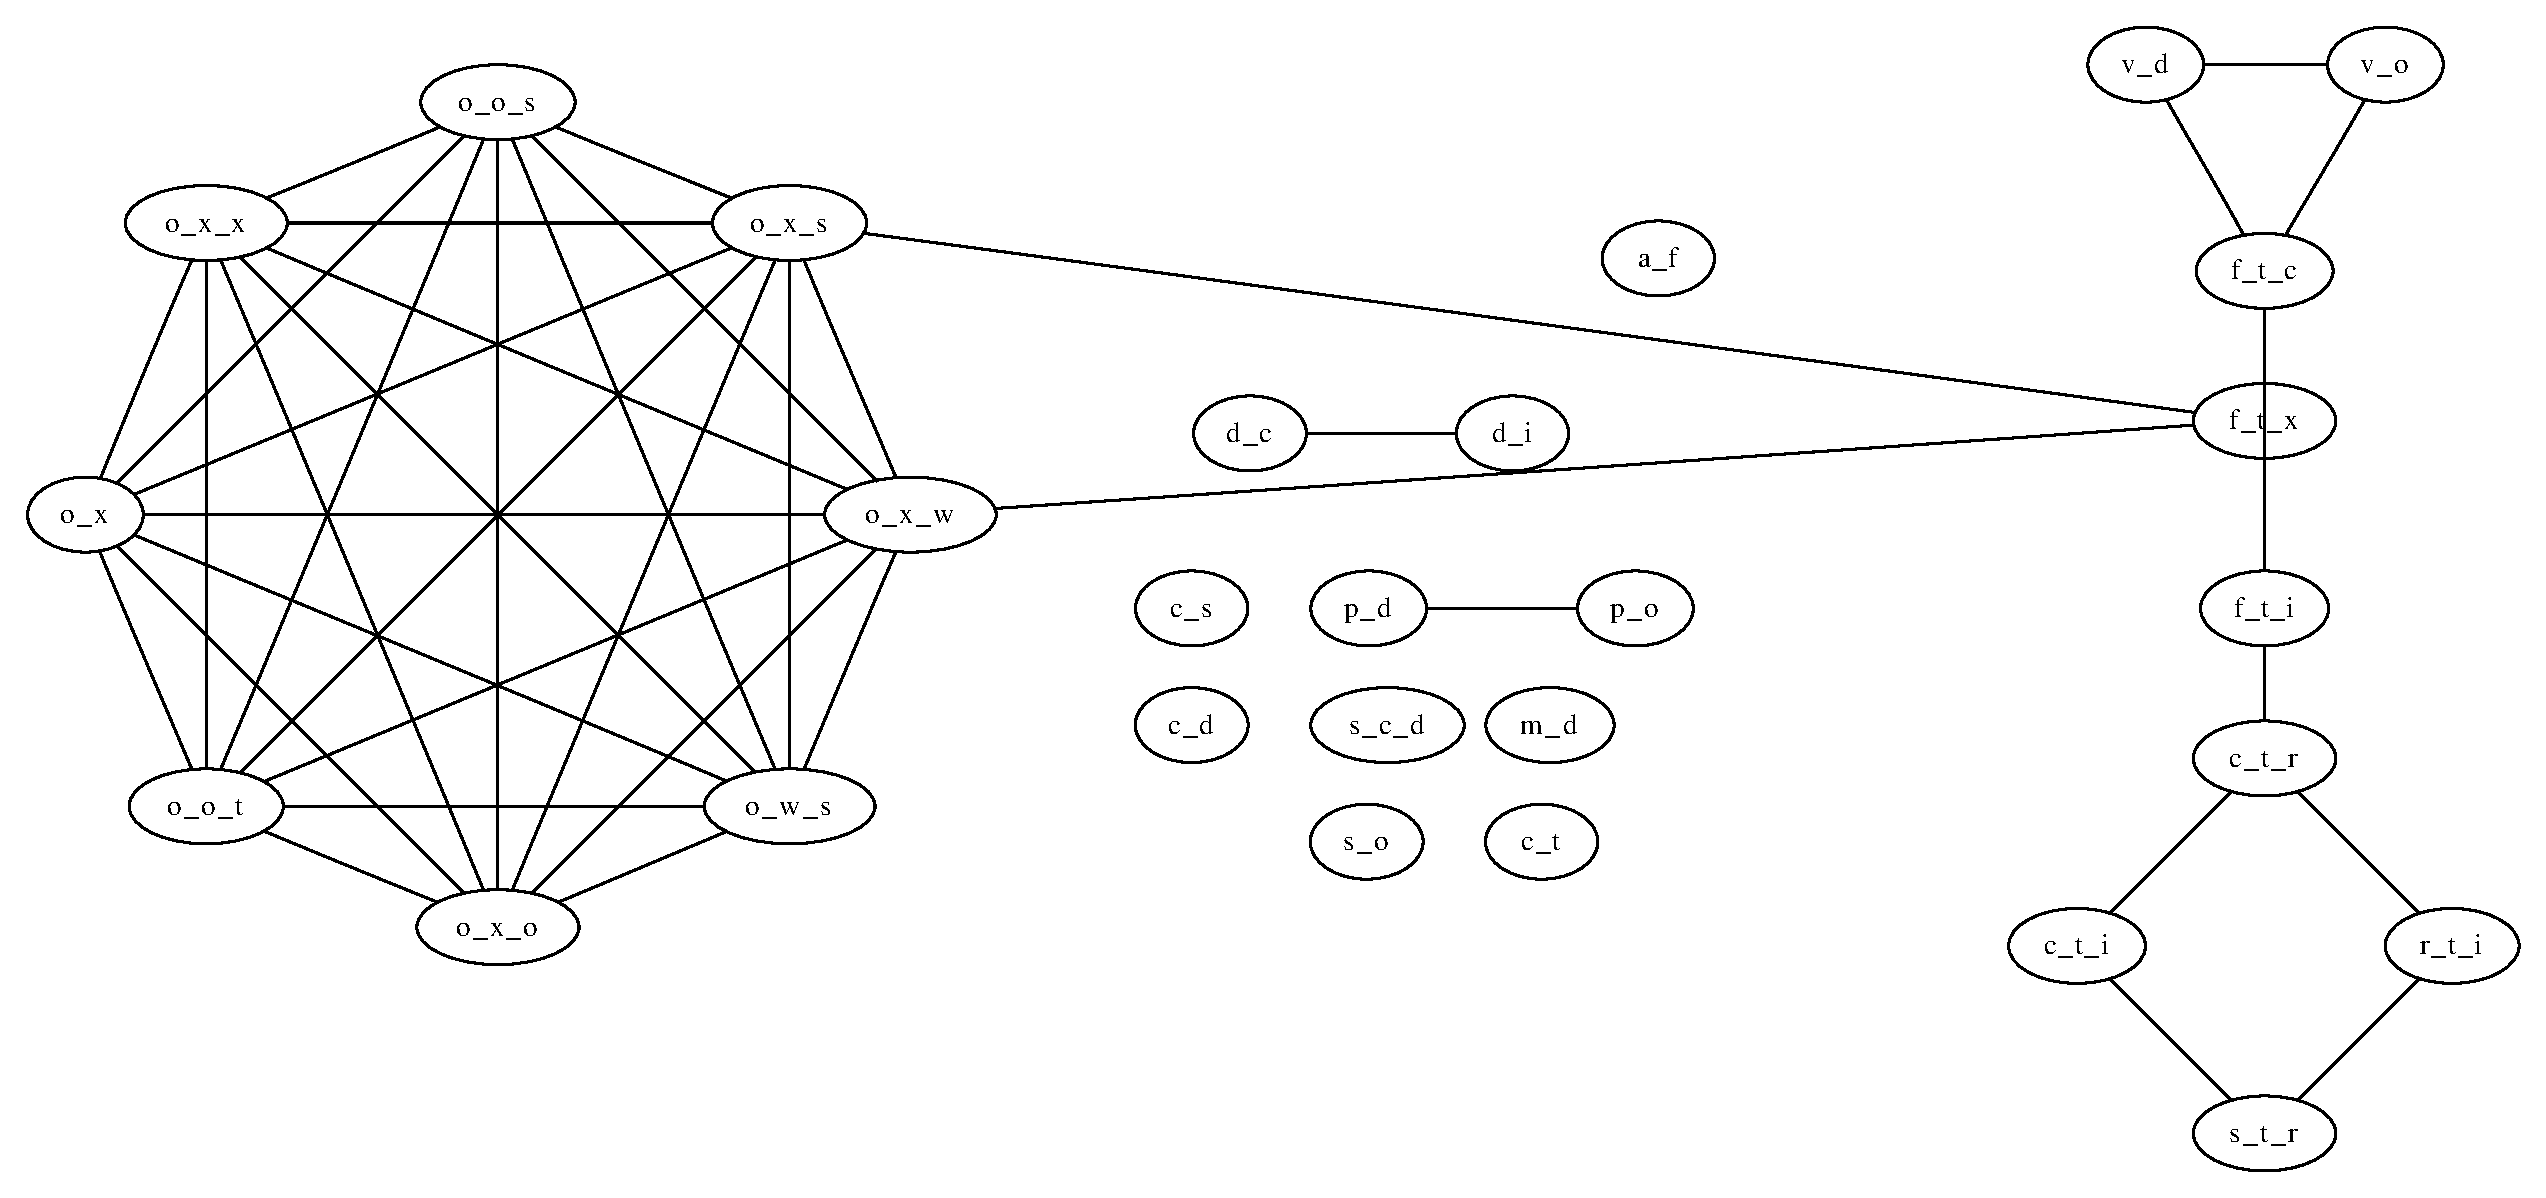
\includegraphics[width=0.45\textwidth]{images/experiments/data/realistic/OVA1}}
    \subfigure[\dataset{OVA2}]{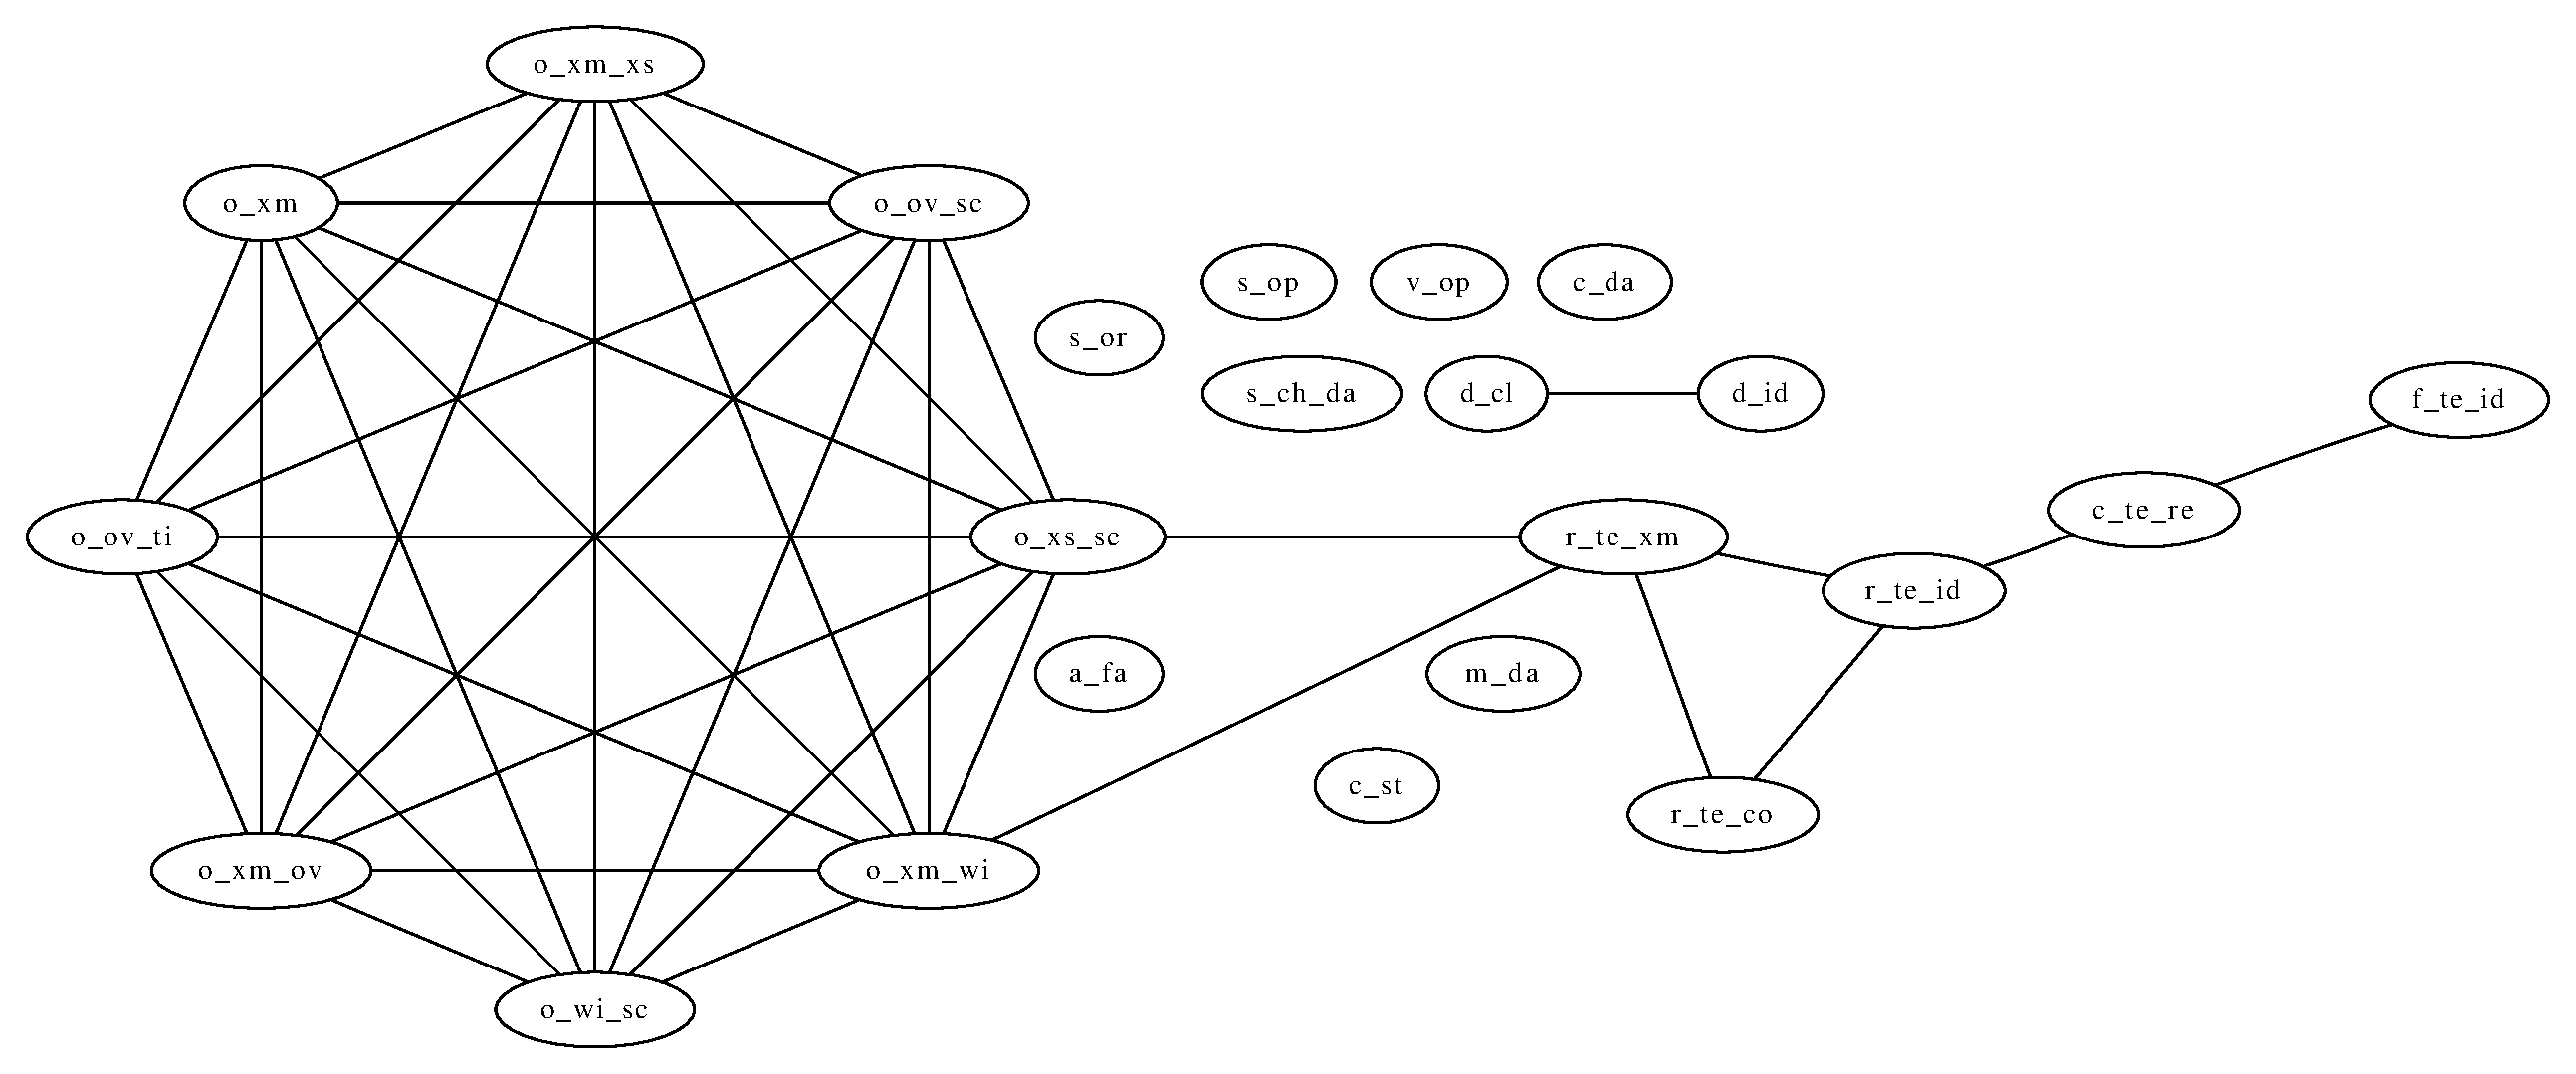
\includegraphics[width=0.45\textwidth]{images/experiments/data/realistic/OVA2}}
    \subfigure[\dataset{OVA3}]{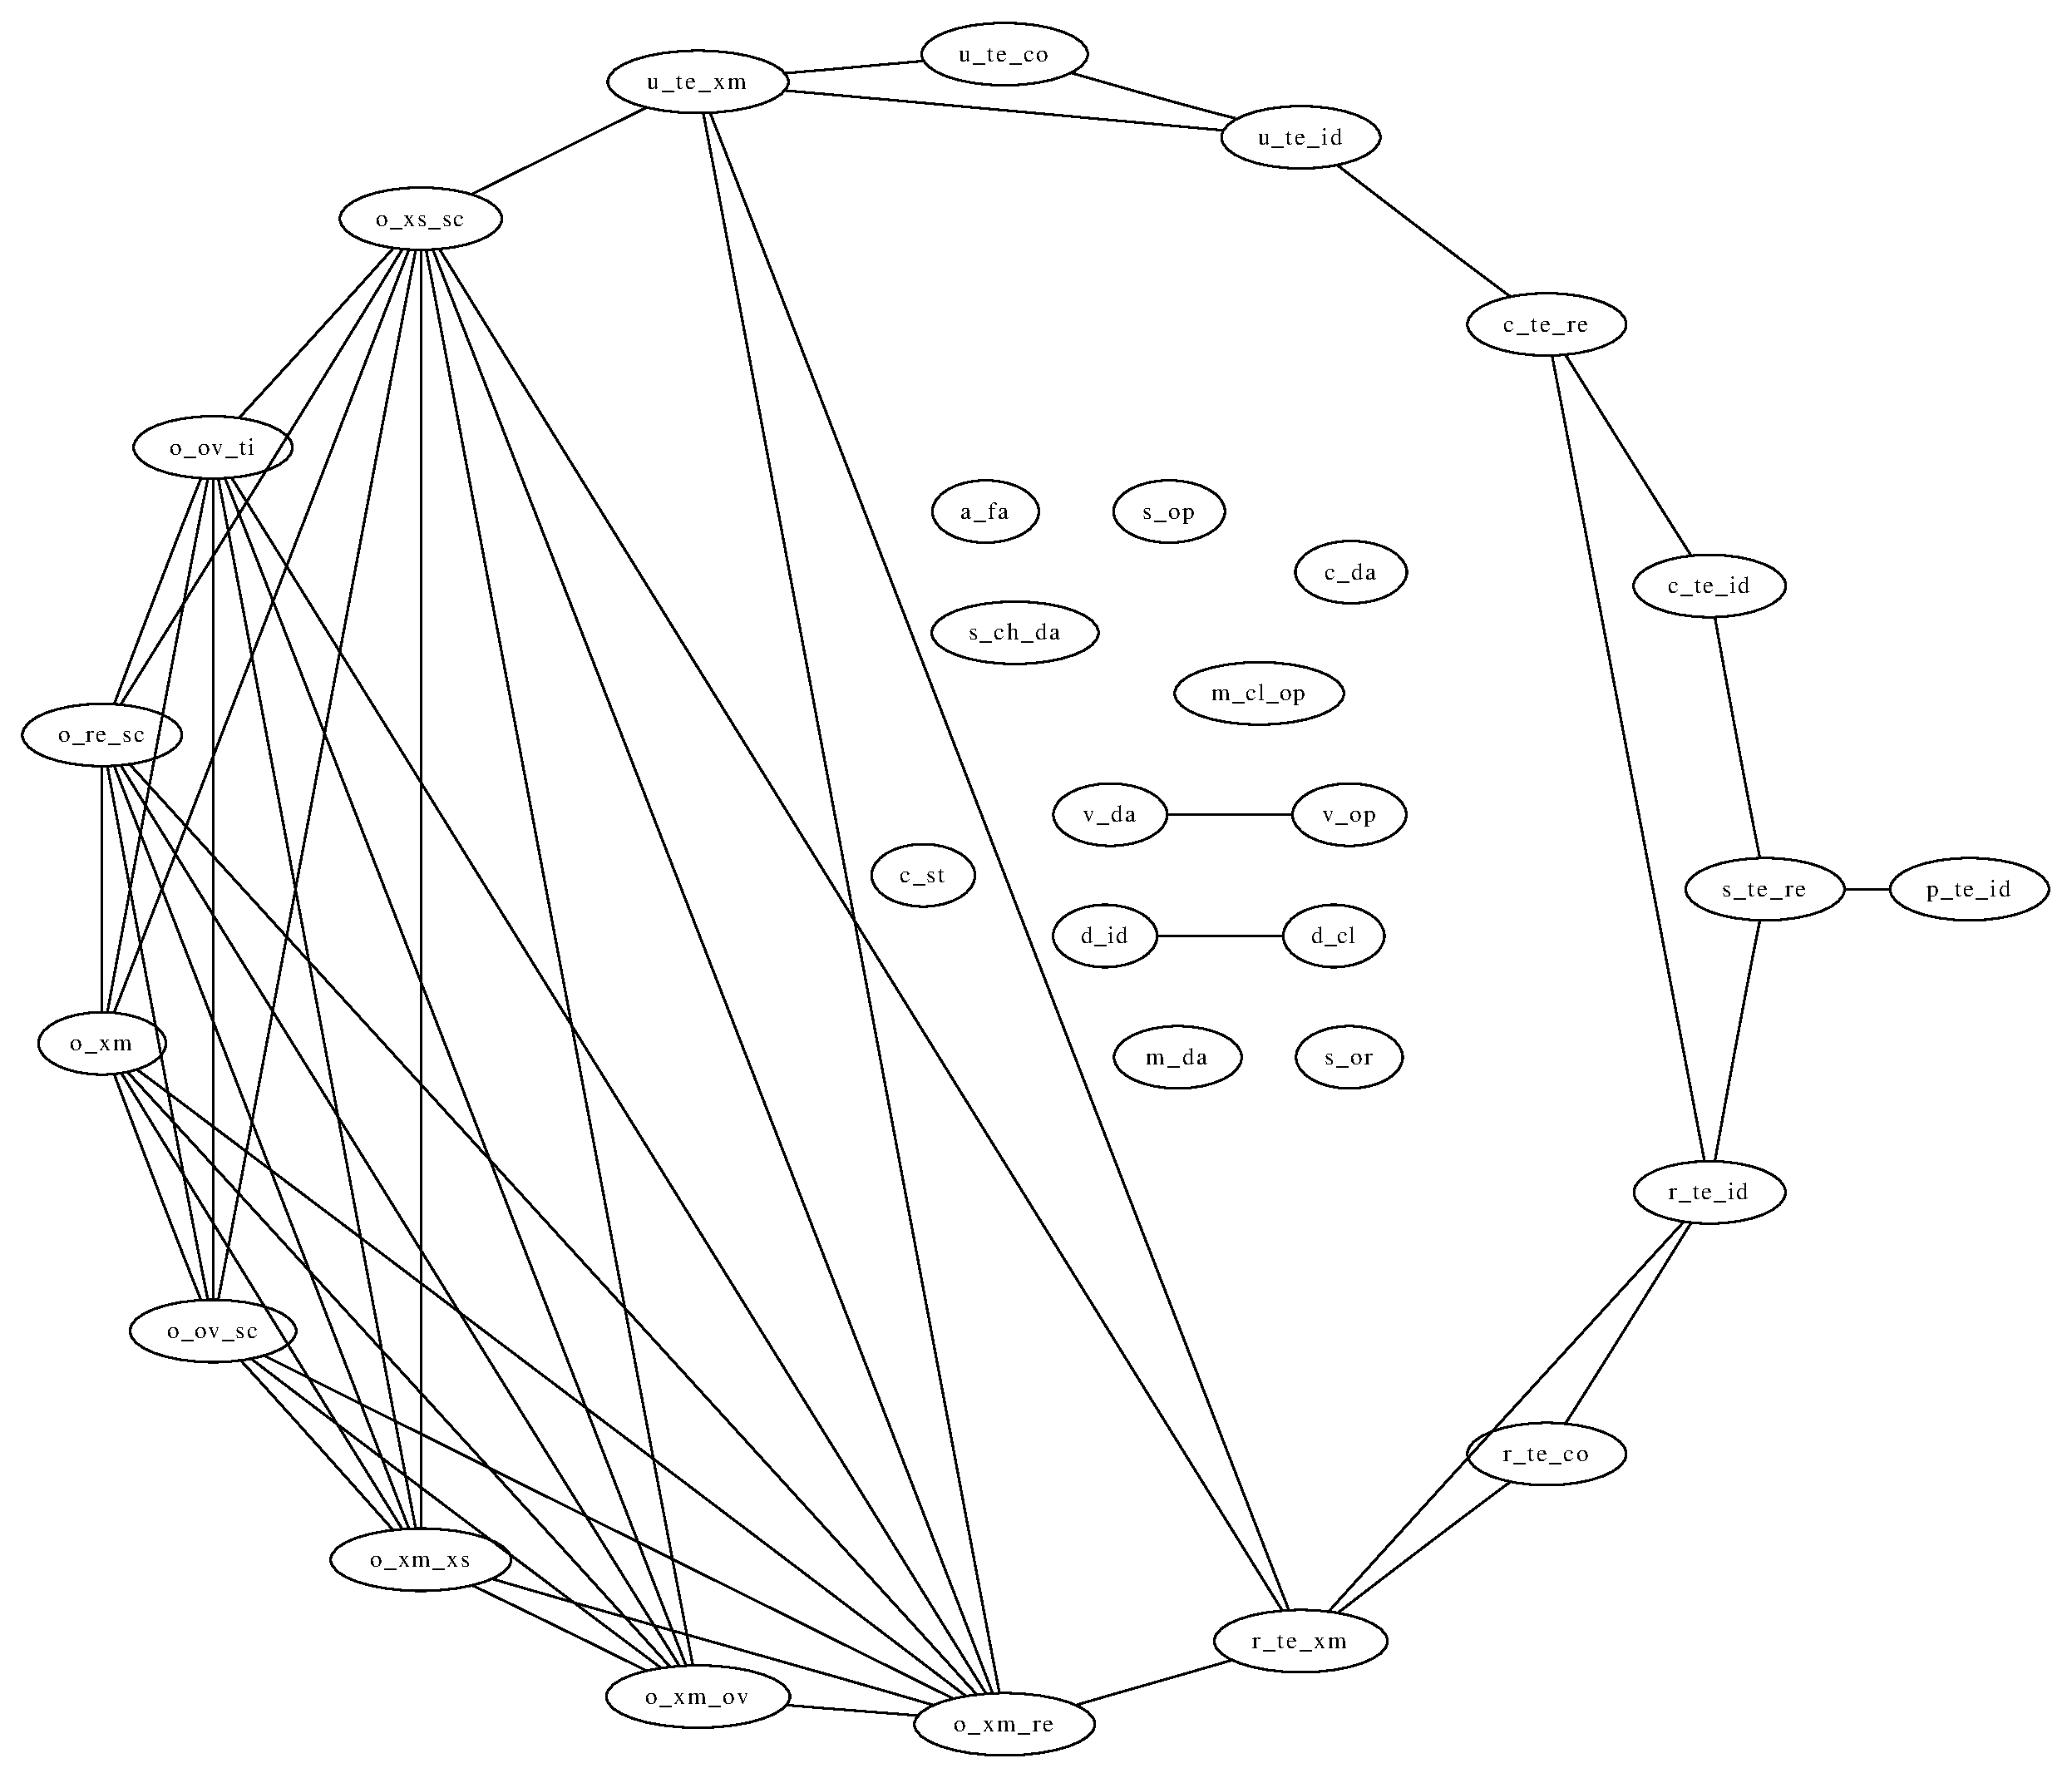
\includegraphics[width=0.45\textwidth]{images/experiments/data/realistic/OVA3}}
    \subfigure[\dataset{XMA-c}]{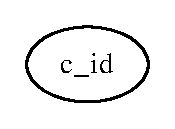
\includegraphics[width=0.08\textwidth]{images/experiments/data/realistic/XMA-c}}
    \subfigure[\dataset{XMA-p}]{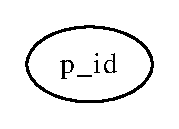
\includegraphics[width=0.08\textwidth]{images/experiments/data/realistic/XMA-p}}
    \subfigure[\dataset{XMD}]{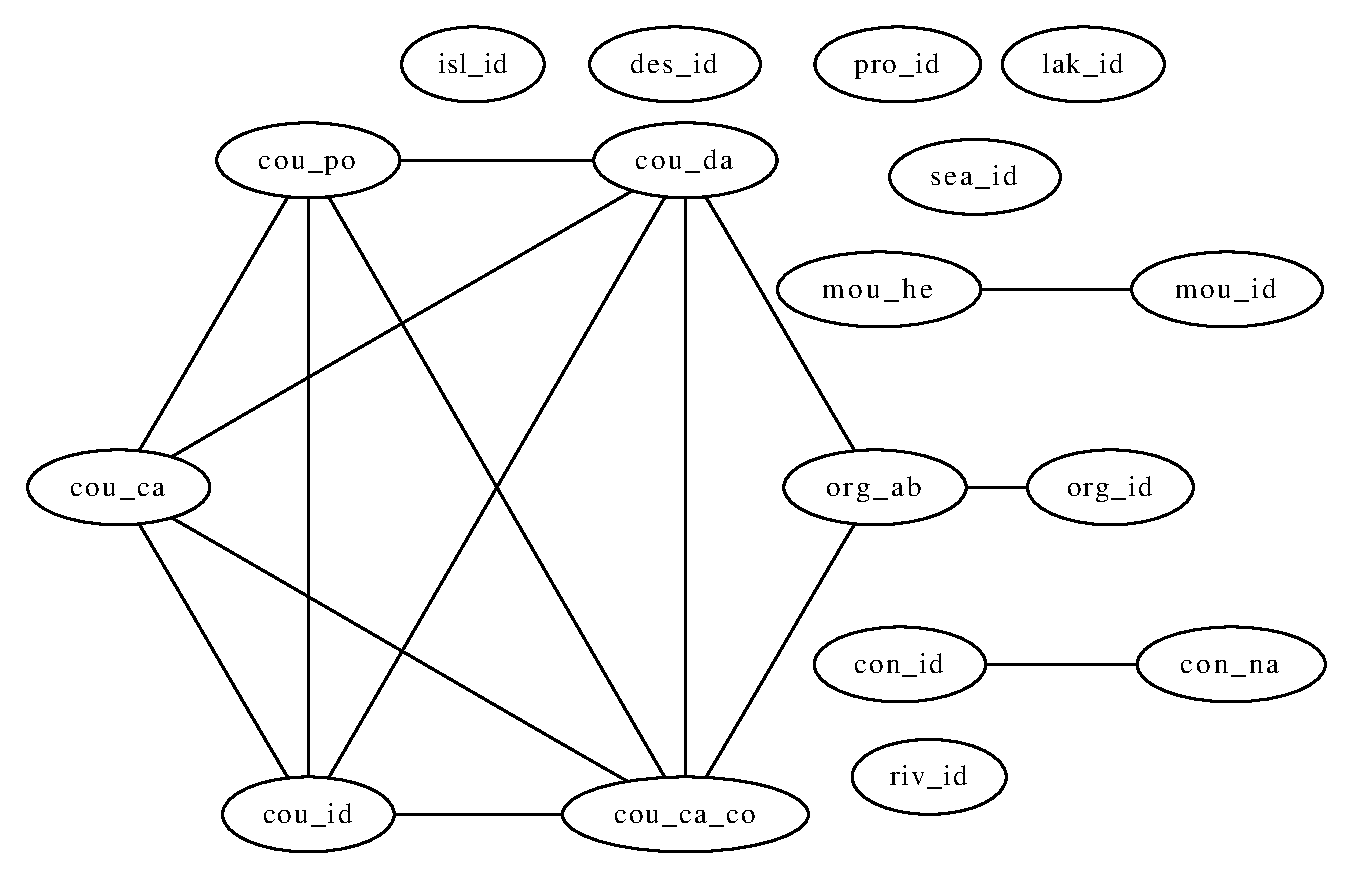
\includegraphics[width=0.45\textwidth]{images/experiments/data/realistic/XMD}}
\end{figure}

To interpret the data a little: \dataset{OVA*} sets have quite interesting and perhaps a bit challenging graphs, but are not too big. We can consider them to be the ``typical" representants.

On the other hand, the \dataset{XMA-*} sets are quite huge, but trivial: their only candidate AM will just get picked and that will be the end of the heuristic. We will see the performance of the other components of the whole system, dealing with huge data that are rather simple in the end.

Finally, the \dataset{XMD} set is quite big and at the same time has non-trivial graph representation. We should see a performance more balanced between processing and finding the ID set here.

\subsection{Realistic data with artificial attributes}
\label{realistic-converted}

We found 2 data sets to convert, \dataset{MSH} and \dataset{NTH}. Unfortunately, the same problem with disclosure as in the previous case applies here. None of these sets had any attributes before the conversion. Their summary is the Table \ref{table-experiments-data-converted}, their graphs can be seen in Figure \ref{image-experiments-data-converted}.

TODO schemas?

To address the conversion: in the case of \dataset{MSH} we found 2 elements with values looking suspiciously like a key of the records contained in the file, and converted them to be attributes of these records using a simple XSL transformation. In the case of \dataset{NTH} we converted all the values in sub-elements of the record elements to be the attributes of the records.

Why is this useful at all? Recall TODO link, where we said that ID attributes are a special case of XML keys. We can use this approach then to find XML keys: convert some suspicious data into attributes, find the optimal ID set and then create XML key based on this ID set.

\begin{table}
  \caption{List of realistic test data files with converted attributes}
  \bigskip
  \label{table-experiments-data-converted}
  \centering
  \begin{tabular}{l | r | c | c | l}
  	Name  & Size [kb] & $|V|$ & $|E|$ & Optimum \\
  	\hline
  	\dataset{MSH}  & 3 100.5 & 1 & 0 & 0.5416472778036296 \\
  	\dataset{NTH}  & 2 523.5 & 5 & 7 & 0.057918595422124436 \\
  \end{tabular}
\end{table}

\begin{figure}
  \caption{Realistic data with converted attributes}
  \label{image-experiments-data-converted}
  \centering
    \subfigure[\dataset{MSH}]{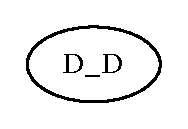
\includegraphics[width=0.08\textwidth]{images/experiments/data/converted/MSH}}
    \subfigure[\dataset{NTH}]{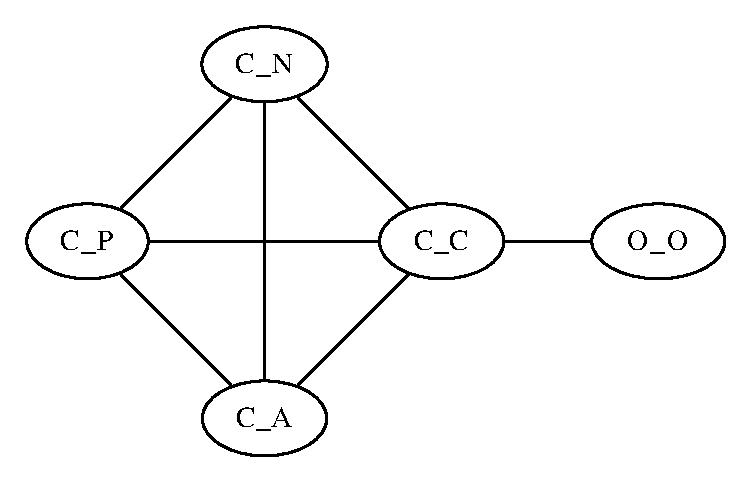
\includegraphics[width=0.45\textwidth]{images/experiments/data/converted/NTH}}
\end{figure}

Again to do a little interpretation: in the case of \dataset{MSH} we created 2 attributes, of which only one constituted a candidate AM. This is then the case similar to \dataset{XMA-*} sets: quite large data, yet only one trivial ID attribute to be found.

In the case of \dataset{NTH} we introduced more attributes, 8 to be precise. Out of them 5 proved to be candidate AMs, with 7 edges constraining them. This means we have quite a big set with relatively simple work to be done by the heuristics. This is about the change.

\subsection{Artificial data}

As soon as we started experimenting with the data coming from the real world, it was obvious that they present no real challenge to our heuristics. After we build the model, we get the most complex graphs of some 31 vertices and 47 edges (see Table \ref{table-experiments-data-realistic}). We needed to create data that would really put pressure on our heuristics, put them to a real test. Our solutions is to approach from the other side: in the end, we will be solving the equivalent of IS problem on a graph created from XML data. Why not create the XML data to contain a more complex graph in the first place? What if we could specify how many vertices and edges we want, and get the according XML?

This is actually simple. Consider the following excerpt from an XML file:

\begin{scriptsize}
\begin{verbatim}
<graph>
  <vertex0 attr="-2968876296119015800"/>
  <vertex1 attr="1729745997570096518"/>
  <vertex2 attr="-9020549659620928934"/>
  ...
  <vertex99 attr="-7545982394508643394"/>

  <vertex82 attr="0"/><vertex21 attr="0"/>
  <vertex64 attr="1"/><vertex21 attr="1"/>
  <vertex44 attr="2"/><vertex2 attr="2"/>
  ...
  <vertex96 attr="99"/><vertex40 attr="99"/>
</graph>
\end{verbatim}
\end{scriptsize}

We want to create a graph with around $v$ vertices and $e$ edges. First, we introduce $v$ elements with names \texttt{vertex0} - \texttt{vertex\{V-1\}}. To constitute an AM, they need an attribute \texttt{attr}, but with large enough random values, so that these values won't conflict with any others. Second, for each of the $e$ edges we pick two \texttt{vertex*} elements at random, and give them the same value of their \texttt{attr}. This will ensure they cannot share the same ID set, thus effectively creating the edge in the graph representation.

The pseudocode for this is in Listing \ref{listing-random-data}.

\begin{algorithm}
\caption{Random XML data creation}
\label{listing-random-data}
\begin{algorithmic}
\REQUIRE $v$ requested number of vertices
\REQUIRE $e$ requested number of edges
\ENSURE XML file content
\PRINT \texttt{<graph>}
\FOR{$i = 1 \to |V|$}
	\STATE $R \gets RANDOM$
	\PRINT \texttt{<vertex\textit{i} attr="\textit{R}">}
\ENDFOR
\FOR{$i = 1 \to |E|$}
	\STATE $v1 \gets RANDOM(|V|)$
	\STATE $v2 \gets RANDOM(|V|)$
	\PRINT \texttt{<vertex\textit{v1} attr="\textit{i}"> <vertex\textit{v2} attr="\textit{i}">}
\ENDFOR
\PRINT \texttt{</graph>}
\RETURN
\end{algorithmic}
\end{algorithm}

With this process in place we can create as much data as we wish with any combination of $v$ and $e$ we want.

There is one interesting characteristic that can describe random graphs like this, and that is the \textit{density}. This can be defined in various ways, we will use two different interpretations for a while. The first is $\frac{|E|}{|V|}$, that is, how many edges are there for one vertex (multiplied by 2 we'd get the average degree of the vertices). The second, perhaps more interesting is $\frac{|E|}{E_{max}}$, where $E_{max} = \frac{|V|.(|V|-1)}{2}$. This is the density as the ratio of edges that are to all edges that could be in a complete graph with $|V|$ vertices.

We have created 3 sets to use in experiments along with the realistic and converted sets, these are called \dataset{100-100}, \dataset{100-200} and \dataset{100-1000}. Note that the name is always in the form $v-e$.\\

All of the experimental data sets mentioned so far, realistic, converted and artificial alike will be referred to as \textit{official test data (sets)}.\\

Also, we will need data of comparably similar characteristics but varying size, to study the effects of size on the run times of experiments. For this reason we created 11 more sets, from \dataset{0-0} as the trivial one to \dataset{100-500} as the biggest one. From now on, these will be referred to as \textit{sized test data (sets)}. We wanted to keep density the same among these sets, and we picked the $\frac{|E|}{E_{max}}$ density interpretation for this.

TODO this is on the DVD.

The summary is the Table \ref{table-experiments-data-artificial} and Table \ref{table-experiments-data-artificial-size}, these tables contain 2 new columns: values of density in both interpretations we introduced. Some graphs can be seen in Figure \ref{image-experiments-data-artificial}.

While studying the tables you might notice that the actual numbers $|V|$ and $|E|$ do not match to the $v$ and $e$ in the names of the sets. This is because how the random generation algorithm works: it might pick the same edge twice, which will automatically render it unsuitable for the ID set (proof is homework). % TODO too much?:)
Because of the so-called Birthday paradox, % TODO link
this will happen more with higher $e$.

\begin{table}
  \caption{List of artificial test data files}
  \bigskip
  \label{table-experiments-data-artificial}
  \centering
  \begin{tabular}{l | r | c | c | c | c | l}
  	Name  & Size [kb] & $|V|$ & $|E|$ & $\frac{|E|}{|V|}$ & $\frac{|E|}{E_{max}}$ & Optimum \\
  	\hline
  	\dataset{100-100}  & 8.4  & 99 & 95  & 0.95 & 0.02 & 0.836666666666667 \\
  	\dataset{100-200}  & 13.0 & 96 & 174 & 1.81 & 0.04 & 0.726000000000000 \\
    \dataset{100-1000} & 49.5 & 93 & 754 & 8.11 & 0.16 & 0.380952380952381 \\
  \end{tabular}
\end{table}

\begin{table}
  \caption{List of ``sized" artificial test data files}
  \bigskip
  \label{table-experiments-data-artificial-size}
  \centering
  \begin{tabular}{l | r | c | c | c | c | l}
	  Name  & Size [kb] & $|V|$ & $|E|$ & $\frac{|E|}{|V|}$ & $\frac{|E|}{E_{max}}$ & Optimum \\
  	\hline
  	\dataset{0-0}     & 0.2  & 0  & 0   & -    & -    & 0.0                \\
  	\dataset{10-5}    & 0.6  & 10 & 5   & 0.50 & 0.11 & 0.8500000000000002 \\
    \dataset{20-20}   & 1.7  & 18 & 13  & 0.72 & 0.08 & 0.7166666666666669 \\
    \dataset{30-45}   & 3.1  & 29 & 43  & 1.48 & 0.11 & 0.7083333333333334 \\
  	\dataset{40-80}   & 5.1  & 39 & 72  & 1.85 & 0.10 & 0.6950000000000002 \\
  	\dataset{50-125}  & 7.5  & 48 & 111 & 2.31 & 0.10 & 0.6566666666666666 \\
  	\dataset{60-180}  & 10.4 & 58 & 157 & 2.71 & 0.09 & 0.6214285714285716 \\
  	\dataset{70-245}  & 13.8 & 67 & 205 & 3.06 & 0.09 & 0.5982142857142856 \\
  	\dataset{80-320}  & 17.6 & 76 & 261 & 3.43 & 0.09 & 0.5791666666666667 \\
  	\dataset{90-405}  & 21.9 & 86 & 352 & 4.09 & 0.10 & 0.528888888888889  \\
  	\dataset{100-500} & 26.7 & 91 & 388 & 4.26 & 0.09 & 0.4981818181818182 \\
  \end{tabular}
\end{table}

\begin{figure}
  \caption{Artificial data}
  \label{image-experiments-data-artificial}
  \centering
  	\subfigure[\dataset{48-80}]{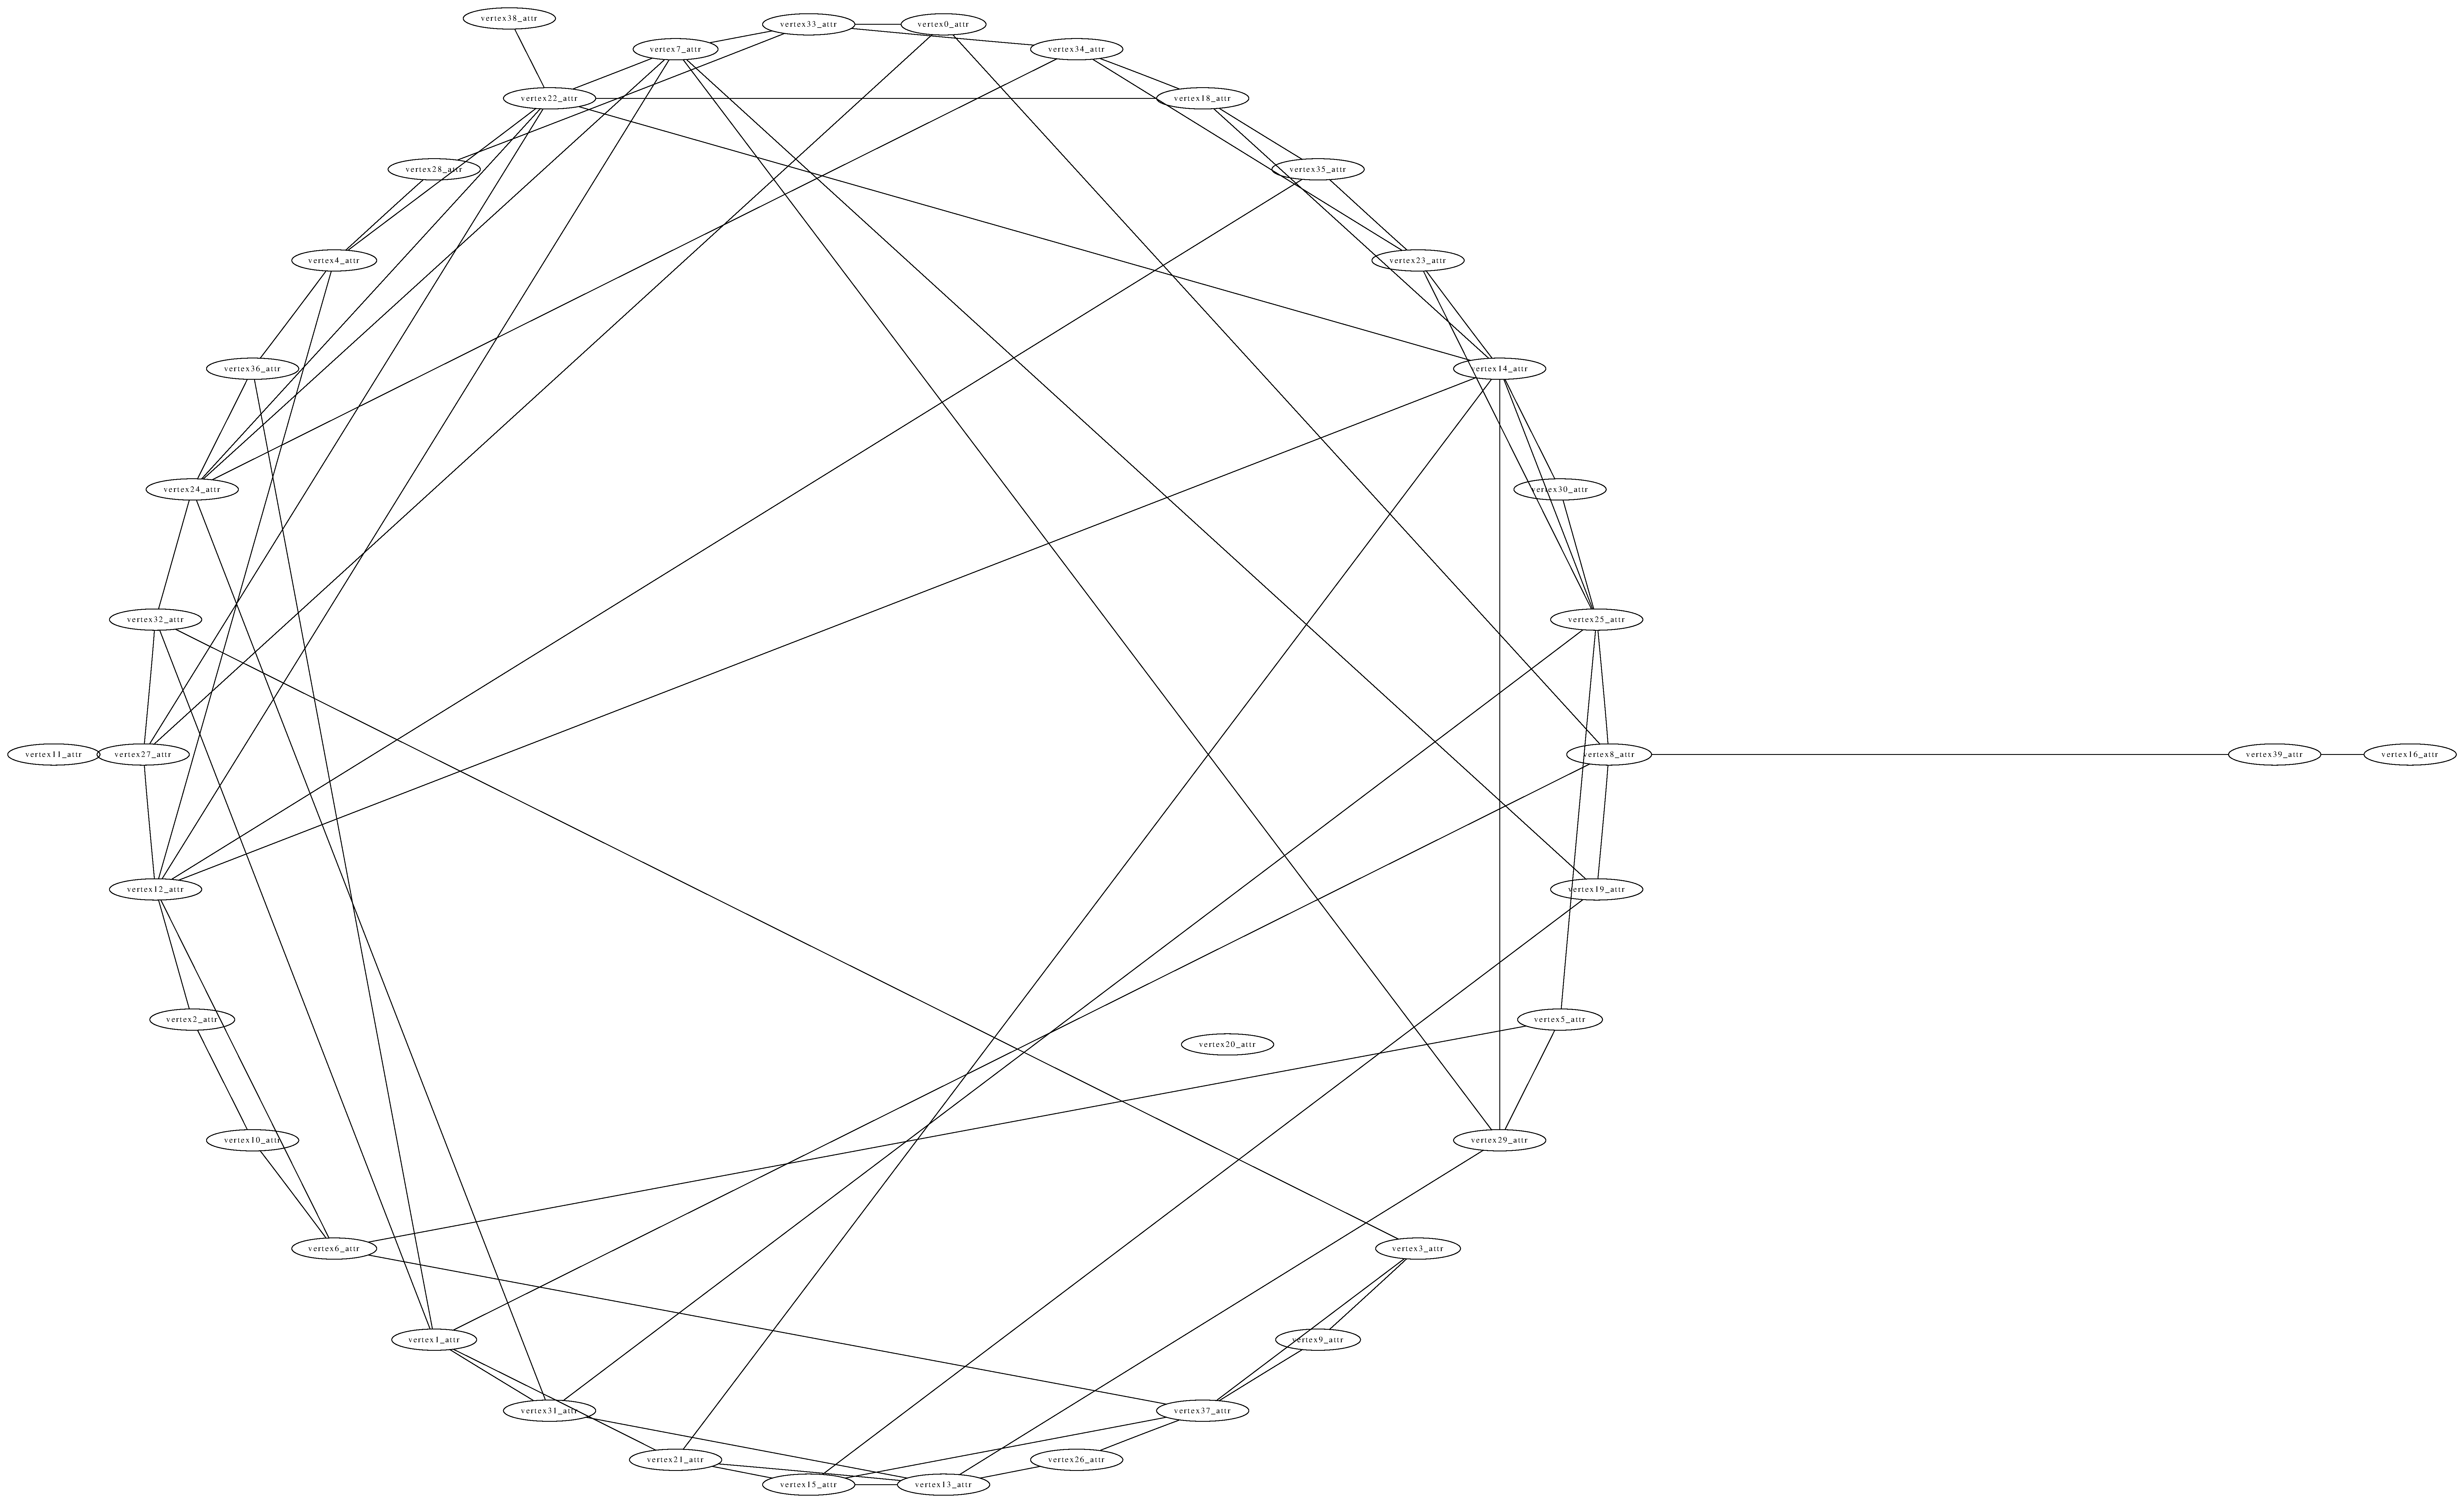
\includegraphics[width=\textwidth]{images/experiments/data/artificial/size/40-80}}
	\subfigure[\dataset{70-245}]{
\includegraphics[width=\textwidth]{images/experiments/data/artificial/size/70-245-fixed}}
\end{figure}

To interpret Tables \ref{table-experiments-data-artificial} and \ref{table-experiments-data-artificial-size}: we get 3 sets of different sizes and densities in the first one, which should work very nice with our heuristics. The $|V|$ and $|E|$ numbers are orders of magnitude higher than with any realistic (or converted) data set we are using, and this will put real stress on the heuristics, as we shall see in the next section.

In the second table we aimed for the $\frac{|E|}{E_{max}}$ density of $0.1 = 10\%$, and we can see that this was quite nicely achieved. There is an interesting observation to be made here: the optimum is steadily decreasing with the increasing overall graph size. This intuitively suggests that the maximal quality theoretically achievable has to do with the $\frac{|E|}{|V|}$ density, not with the one we fixed. Exploration of this phenomenon is among the possibilities of future work of this thesis.

\section{Experimental Setup}

As was mentioned before, we will be using an extension to the jInfer framework called \jmodule{IDSetSearch}. Please see appendices \ref{appendix-jInfer} and \ref{appendix-iss} for more detailed information on these two pieces of software.\\

We now have to define a few notions before moving forward to the description of our experiments.

\begin{define}[Experiment parameters]
	\label{define-experiment-params}
	\textit{Experiment parameters} are the following.
	\begin{itemize}
		\item All the parameters in all the heuristics.
		\item The specific way in which the heuristics are chained.
		\item Parameters $\alpha$ and $\beta$ in the weight (quality) measurement.
		\item Initial pool size.
		\item The termination criteria.
		\item The input XML file.
		\item Known optimum for this file and $\alpha$, $\beta$.
	\end{itemize}
\end{define}

\begin{define}[Experiment(al) configuration]
	\label{define-experiment-config}
	An \textit{experiment instance}, or \textit{configuration}, is one specific setting of all (experiment) parameters.
\end{define}

\begin{define}[Experiment(al) set]
	\label{define-experiment-set}
	One or more experiment configurations, regardless whether their parameters differ, constitute an \textit{experimental set}.
\end{define}

\subsection{Grammar and Model Creation}

TODO link BasicIGG to see how we get IG

TODO describe how we get the model

\subsection{Hardware and Software}

We will be using two different machines to run the experiments. Every experimental result will have explicitly stated the machine it was performed on, and we shall make sure to run different experiments that can benefit from side-by-side comparison on the same machine.

\subsubsection{Quad Core Machine}

\begin{verbatim}
Intel Core 2 Quad processor @ 2.83 GHz
8 GB DDR2 RAM
Windows 7 SP1 64bit
TODO
TODO
GLPK version TODO
\end{verbatim}

\subsubsection{Dual Core Machine}

\begin{verbatim}
Intel Core 2 Duo processor @ 2.33 GHz
4 GB DDR2 RAM
Windows 7 SP1 64bit
Java SE Runtime Environment (build 1.6.0_26-b03)
Java HotSpot 32-Bit Client VM (build 20.1-b02)
GLPK version 4.45 (Cygwin)
GLPK version 4.34 (native)
\end{verbatim}

\subsection{Methodology}

It is impossible to completely shield an experiment from the influence of the environment, but we should try our best. First of all, NetBeans running the experiments is the only relevant program running in the system at that time, as far as this is possible. Unfortunately, the NetBeans itself is quite a large environment with a life on its own, and we would most certainly get more reliable results, if we could run our experiments outside it. This improvement is left for the future work.

Also, every experimental configuration is run 20 times in hope that the effects of any events adversely affecting our results (e.g. OS deciding to run some house cleaning) will be averaged out. Whenever possible, we will always be using boxplots instead of a simple average (or average and variance) to present results of these multiple runs. % TODO discuss caches and the order in which we run the experiments in one set?

\subsection{Measuring the time}

TODO

\subsection{Obtaining the results}

Every run of an experiment produces a trace such as the one presented and commented on in Appendix \ref{appendix-trace}. We can get all the information relevant to that experiment run from this trace alone. An experimental set will produce a number of these traces and store them in plain text files in a folder. Parsing these files to aggregate and collate them might be a tedious task even using tools like \texttt{sed} and \texttt{grep}, so some of the experiment sets directly output tabular data in format recognized by GnuPlot, which we use to plot charts found in this work.

TODO explain boxplots, how to read them

\section{Experimental Results}

\subsection{Grammar and model generation}

%         NB class GrammarModelTiming

The first experiment set will try to establish how long it takes to extract the IG % TODO IG -> nomenclature
from the input XML file and how long does it take to create the AM model from this IG. For now, we will not be running or measuring any heuristics.

\begin{center}
\bigskip
\begin{tabular}{| l | l |}
  \hline
  \hline
  Machine           & Dual Core \\
  Input data        & all official and sized test data sets \\
  Iterations        & 50 \\
  Pool size         & not applicable \\
  $\alpha$, $\beta$ & not applicable \\
  \hline
\end{tabular}
\bigskip
\end{center}

The experimental set will contain $50 * (11 + 11) = 1100$ configurations: 20 iterations for 11 test data sets plus 11 sized test data sets. There will be no CHs or IHs. We will be gathering the timing data for IG extraction and model generation in GnuPlot format.

\begin{table}
  \caption{Grammar Extraction and Model Creation Times}
  \bigskip
  \label{table-experiments-grammar-model-timing}
  \centering
  \begin{tabular}{l || l | l || l | l || l | l}
    Data set & GE & GE & MC & MC & Tot & Tot \\
     & avg [ms] & stdev & avg [ms] & stdev & avg [ms] & stdev \\
    \hline
    \dataset{OVA1}     & < 10 & - & < 10 & - < 10 & - \\
    \dataset{OVA2}     & < 10 & - & < 10 & - < 10 & - \\
    \dataset{OVA3}     & 42.94 & 19.8509 & 60.92 & 27.0848 & 103.86	& 31.6911 \\
    \dataset{XMA-c}    & 140.32 &	33.2618 &	90.24 &	45.8803 & 230.56 & 56.2633 \\
	\dataset{XMA-p}    & 7518.82 &	922.8882 &	10135.46 &	502.8997 & 17654.28	& 1353.8794 \\
	\dataset{XMD}      & 979.18 &	307.1760 &	563.04 & 341.4697 & 1542.22	& 134.6883 \\
	\dataset{MSH}      & 570.24 &	167.1119 &	225.48 &	90.6775 & 795.72 & 161.8340 \\ 
	\dataset{NTH}      & 328.36 & 118.3766 &	1074.9 &	155.5604 & 1403.26 & 137.8695 \\
	\dataset{100-100}  & < 10 & - & < 10 & - & < 10 & - \\
	\dataset{100-200}  & < 10 & - & < 10 & - & < 10 & - \\
	\dataset{100-1000} & 18.34 & 10.2372 & 18.84 & 1.0373 & 37.18 & 9.9338 \\
	\dataset{0-0}      & < 10 & - & < 10 & - & < 10 & - \\
	\dataset{10-5}     & < 10 & - & < 10 & - & < 10 & - \\
	\dataset{20-20}    & < 10 & - & < 10 & - & < 10 & - \\
	\dataset{30-45}    & < 10 & - & < 10 & - & < 10 & - \\
	\dataset{40-80}    & < 10 & - & < 10 & - & < 10 & - \\
	\dataset{50-125}   & < 10 & - & < 10 & - & < 10 & - \\
	\dataset{60-180}   & < 10 & - & < 10 & - & < 10 & - \\
	\dataset{70-245}   & < 10 & - & < 10 & - & < 10 & - \\
	\dataset{80-320}   & < 10 & - & < 10 & - & 12.48 & 8.3574 \\
	\dataset{90-405}   & < 10 & - & < 10 & - & 15.88 & 10.3778 \\
	\dataset{100-500}  & < 10 & - & < 10 & - & 18.74 &	8.8889 \\
  \end{tabular}
\end{table}

TODO interpretation

\subsubsection{GLPK interface timing}

%         NB class GlpkInterfaceTiming

A related problem is how long it takes to create input for GLPK and then parse its results. We will use the same test data sets as in the previous case, but now we will gather times needed to communicate with GLPK.

\begin{table}
  \caption{GLPK Interface Times}
  \bigskip
  \label{table-experiments-glpk-timing}
  \centering
  \begin{tabular}{l || l | l || l | l || l | l}
	Data set & IC & IC & OP & OP & Tot & Tot \\
     & avg [ms] & stdev & avg [ms] & stdev & avg [ms] & stdev \\
	\hline
	\dataset{OVA1} & 36.46 & 66.8517 & 49.8 & 114.0687 & 86.26 & 150.1044 \\
	\dataset{OVA2} & 39.52 & 75.8210 & 48.8 & 102.4484 & 88.32 & 154.9596 \\
	\dataset{OVA3} & 34.1 & 74.1838 & 38.62 & 89.3772 & 72.72 & 134.7295 \\
	\dataset{XMA-c} & 40.88 & 88.6632 & 33.84 & 65.8636 & 74.72 & 127.7338 \\
	\dataset{XMA-p} & 36.54 & 70.7436 & 49.24 & 101.2412 & 85.78 & 145.2092 \\
	\dataset{XMD} & 37.98 & 69.2719 & 32.88 & 70.2173 & 70.86 & 114.6692 \\
	\dataset{MSH} & 40.42 & 91.9885 & 36.52 & 72.1018 & 76.94 & 138.6198 \\
	\dataset{NTH} & 36.02 & 66.3403 & 38.06 & 88.8244 & 74.08 & 128.9974 \\
	\dataset{100-100} & 46.5 & 103.3929 & 46.92 & 89.7049 & 93.42 & 158.7267 \\
	\dataset{100-200} & 42.34 & 96.1204 & 38.22 & 90.0284 & 80.56 & 152.6534 \\
	\dataset{100-1000} & 32.92 & 64.4534 & 42.1 & 89.4546 & 75.02 & 127.8541 \\
	\dataset{0-0} & 46.8 & 123.5183 & 46.92 & 102.2601 & 93.72 & 181.5228 \\
	\dataset{10-5} & 40.06 & 75.7370 & 40.1 & 72.4851 & 80.16 & 126.7135 \\
	\dataset{20-20} & 33.72 & 70.7263 & 34.1 & 66.2781 & 67.82 & 116.3783 \\
	\dataset{30-45} & 38.26 & 71.7549 & 45.94 & 110.1284 & 84.2 & 155.7594 \\
	\dataset{40-80} & 37.06 & 67.0024 & 49.26 & 106.3185 & 86.32 & 144.9918 \\
	\dataset{50-125} & 50.44 & 101.9162 & 84.76 & 364.7350 & 135.2 & 378.7835 \\
	\dataset{60-180} & 38.38 & 89.3379 & 42.54 & 94.3742 & 80.92 & 149.6049 \\
	\dataset{70-245} & 41.5 & 93.2951 & 40.3 & 93.4858 & 81.8 & 149.6797 \\
	\dataset{80-320} & 51.92 & 121.9812 & 47.98 & 96.0904 & 99.9 & 171.4617 \\
	\dataset{90-405} & 40.5 & 91.5373 & 36.46 & 88.5099 & 76.96 & 144.2890 \\
	\dataset{100-500} & 37.82 & 85.7571 & 43.4 & 90.3257 & 81.22 & 141.9103 \\
  \end{tabular}
\end{table}

TODO interpretation: it is interesting that even though $|V|$ and $|E|$ are increasing, the times remain almost the same. This probably means that the most of the time is spent in I/O.

\subsection{GLPK: native vs. Cygwin}

%         NB class TimeQuality
%         NB class TimeTillOptimum

In this experiment we will try to remove one of the variables out of the equation: that is the effect of different versions of GLPK on the overall results. The rationale is this: on Windows systems, the two most accessible ways to install GLPK are via a binary distribution TODO link, or via Cygwin as one of its packages.

If we find out which of these Cygwin version is better, we will be using it exclusively without very much fear that this could affect any other aspect of our experiments. We might also find that there is no relevant difference, which would be good, too.

Apart from comparing different versions, we shall see how the pure GLPK approach behaves. The first part of this experiment will be limiting the run time, thus making it an instance of Truncated branch \& bound. In this case we will see the dependency between the run time and the quality achieved in it. In the second time we will let GLPK run until optimum is found. We shall see the dependency between input size and run time needed to achieve the optimum.

\begin{center}
\bigskip
\begin{tabular}{| l | l |}
  \hline
  \hline
  Machine           & Dual Core \\
  Input data        & \dataset{100-500} \\
  Iterations        & 50 \\
  Pool size         & 1 \\
  $\alpha$, $\beta$ & $1$, $1$ \\
  \hline
\end{tabular}
\bigskip
\end{center}

Our experimental set will contain 500 experimental configurations for each of these two GLPK version. Every configuration will use \heu{Glpk} CH set to a time limit from 1 to 46 seconds with increments of 5, meaning 10 settings * 50 iterations = 500 configurations in total (see Listing \ref{listing-experiment-glpk-native-vs-cygwin-1}). There will be no improvement heuristic. The only data we gather in the GnuPlot file are the final qualities (weights).

\begin{algorithm}
\caption{GLPK: native vs. Cygwin set generation 1}
\label{listing-experiment-glpk-native-vs-cygwin-1}
\begin{algorithmic}
\ENSURE experimental set $ES$
\STATE $ES \gets \emptyset$
\FOR{$i = 1 \to 50$}
	\FOR{$time = 1 \to 49$ step $2$}
    \STATE $ES \gets ES \cup {CH = \heu{Glpk}(limit = time), IH = \emptyset}$
  \ENDFOR
\ENDFOR
\RETURN $ES$
\end{algorithmic}
\end{algorithm}

\begin{figure}
  \caption{Time vs. Quality}
  \label{image-experiment-time-vs-quality}
  \centering
    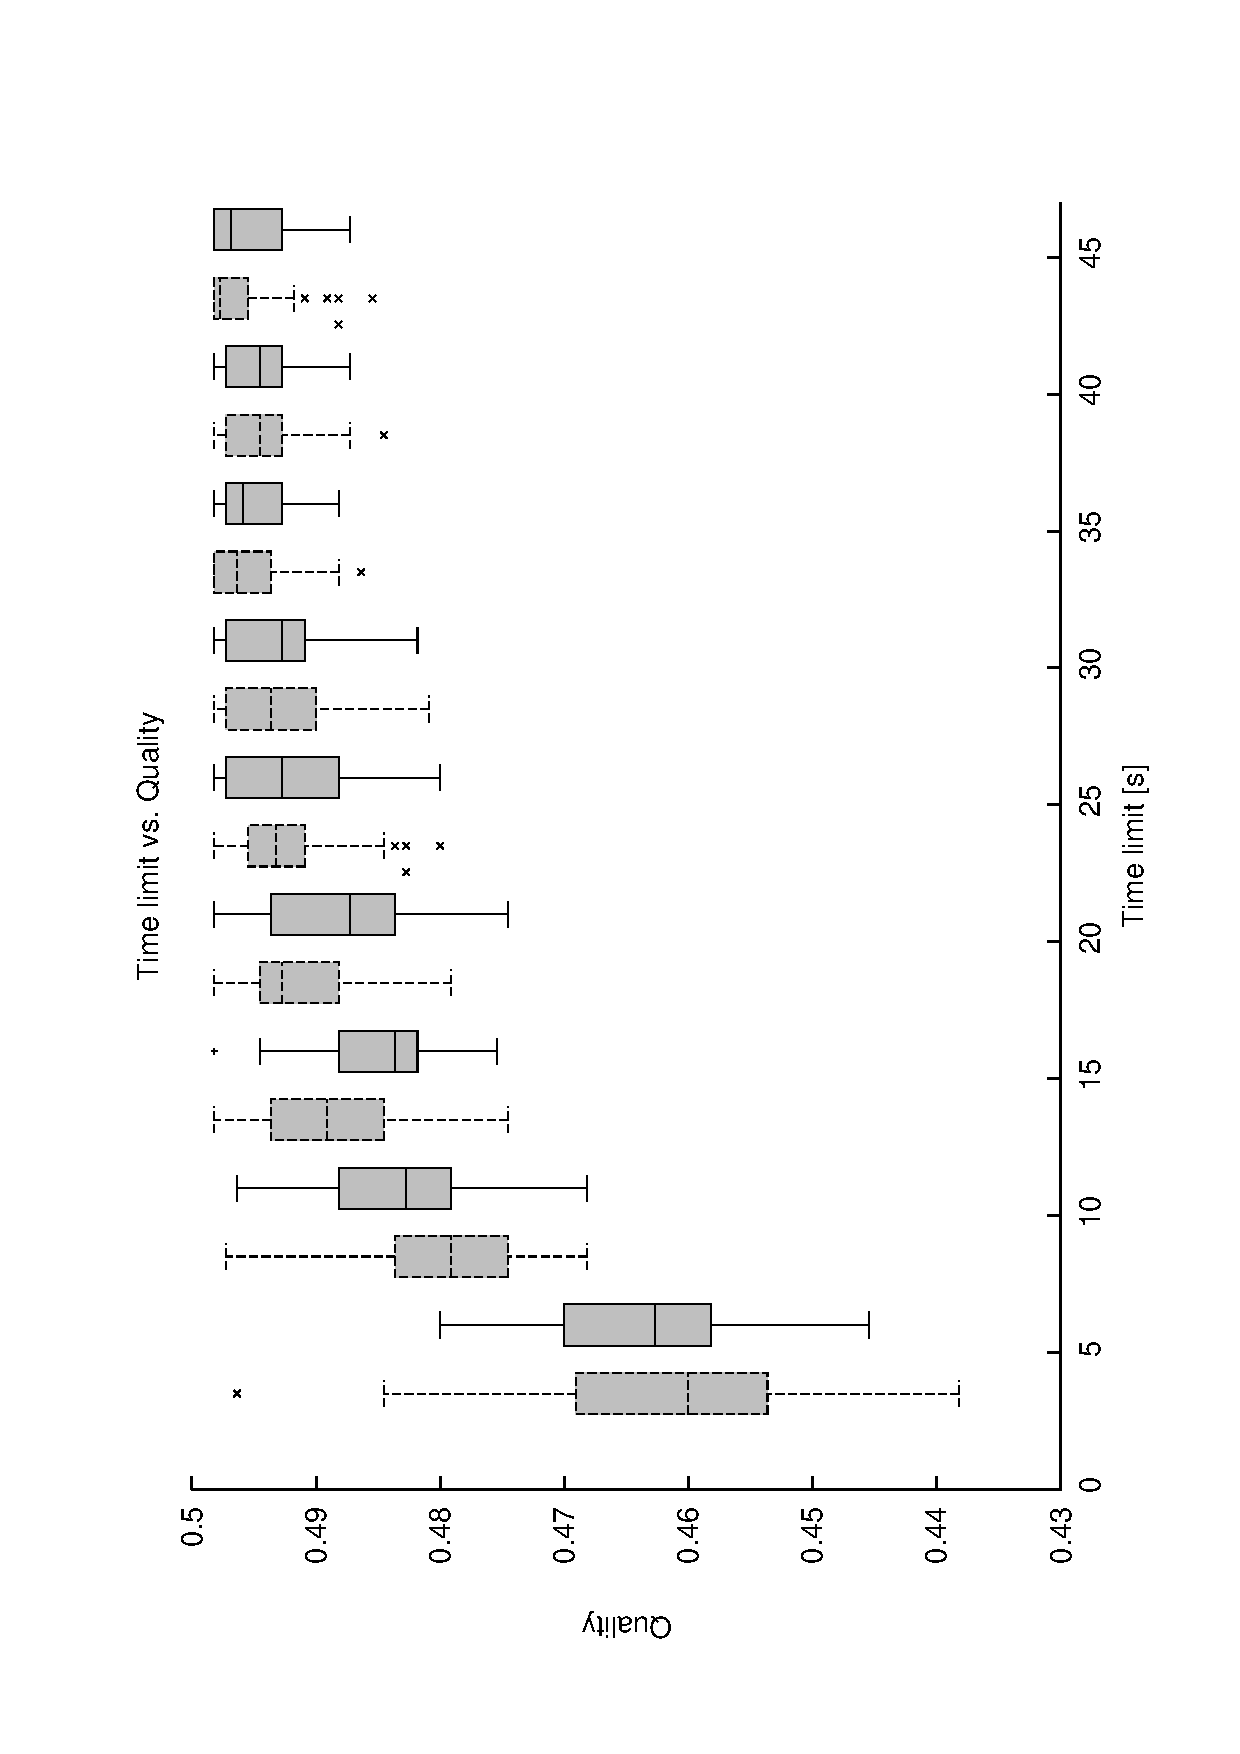
\includegraphics[width=\textwidth]{images/experiments/time-vs-quality}
\end{figure}

TODO interpretation

\begin{center}
\bigskip
\begin{tabular}{| l | l |}
  \hline
  \hline
  Machine           & Dual Core \\
  Input data        & all sized test data sets \\
  Iterations        & 50 \\
  Pool size         & 1 \\
  $\alpha$, $\beta$ & $1$, $1$ \\
  \hline
\end{tabular}
\bigskip
\end{center}

Another way to compare the performance of these two GLPK versions is to see how long it takes them to find the optimum for a set of data of increasing size. This experimental set will contain 220 configurations for each version. Every configuration will let \heu{Glpk} CH run for unlimited time, until it finds the optimum. This will be repeated in 20 iterations for each of the 11 files from the sized test data set (see Listing \ref{listing-experiment-glpk-native-vs-cygwin-2}). There will again be no IH, the only data we will collect are the times of the CH run in each case.

\begin{algorithm}
\caption{GLPK: native vs. Cygwin set generation 2}
\label{listing-experiment-glpk-native-vs-cygwin-2}
\begin{algorithmic}
\ENSURE experimental set $ES$
\STATE $ES \gets \emptyset$
\FOR{$i = 1 \to 20$}
	\FOR{$file \in $ sized test data}
    \STATE $ES \gets ES \cup \{file, CH = \heu{Glpk}(no\:limit), IH = \emptyset\}$
  \ENDFOR
\ENDFOR
\RETURN $ES$
\end{algorithmic}
\end{algorithm}

\begin{figure}
  \caption{Time Until Optimum}
  \label{image-experiment-time-until-optimum}
  \centering
    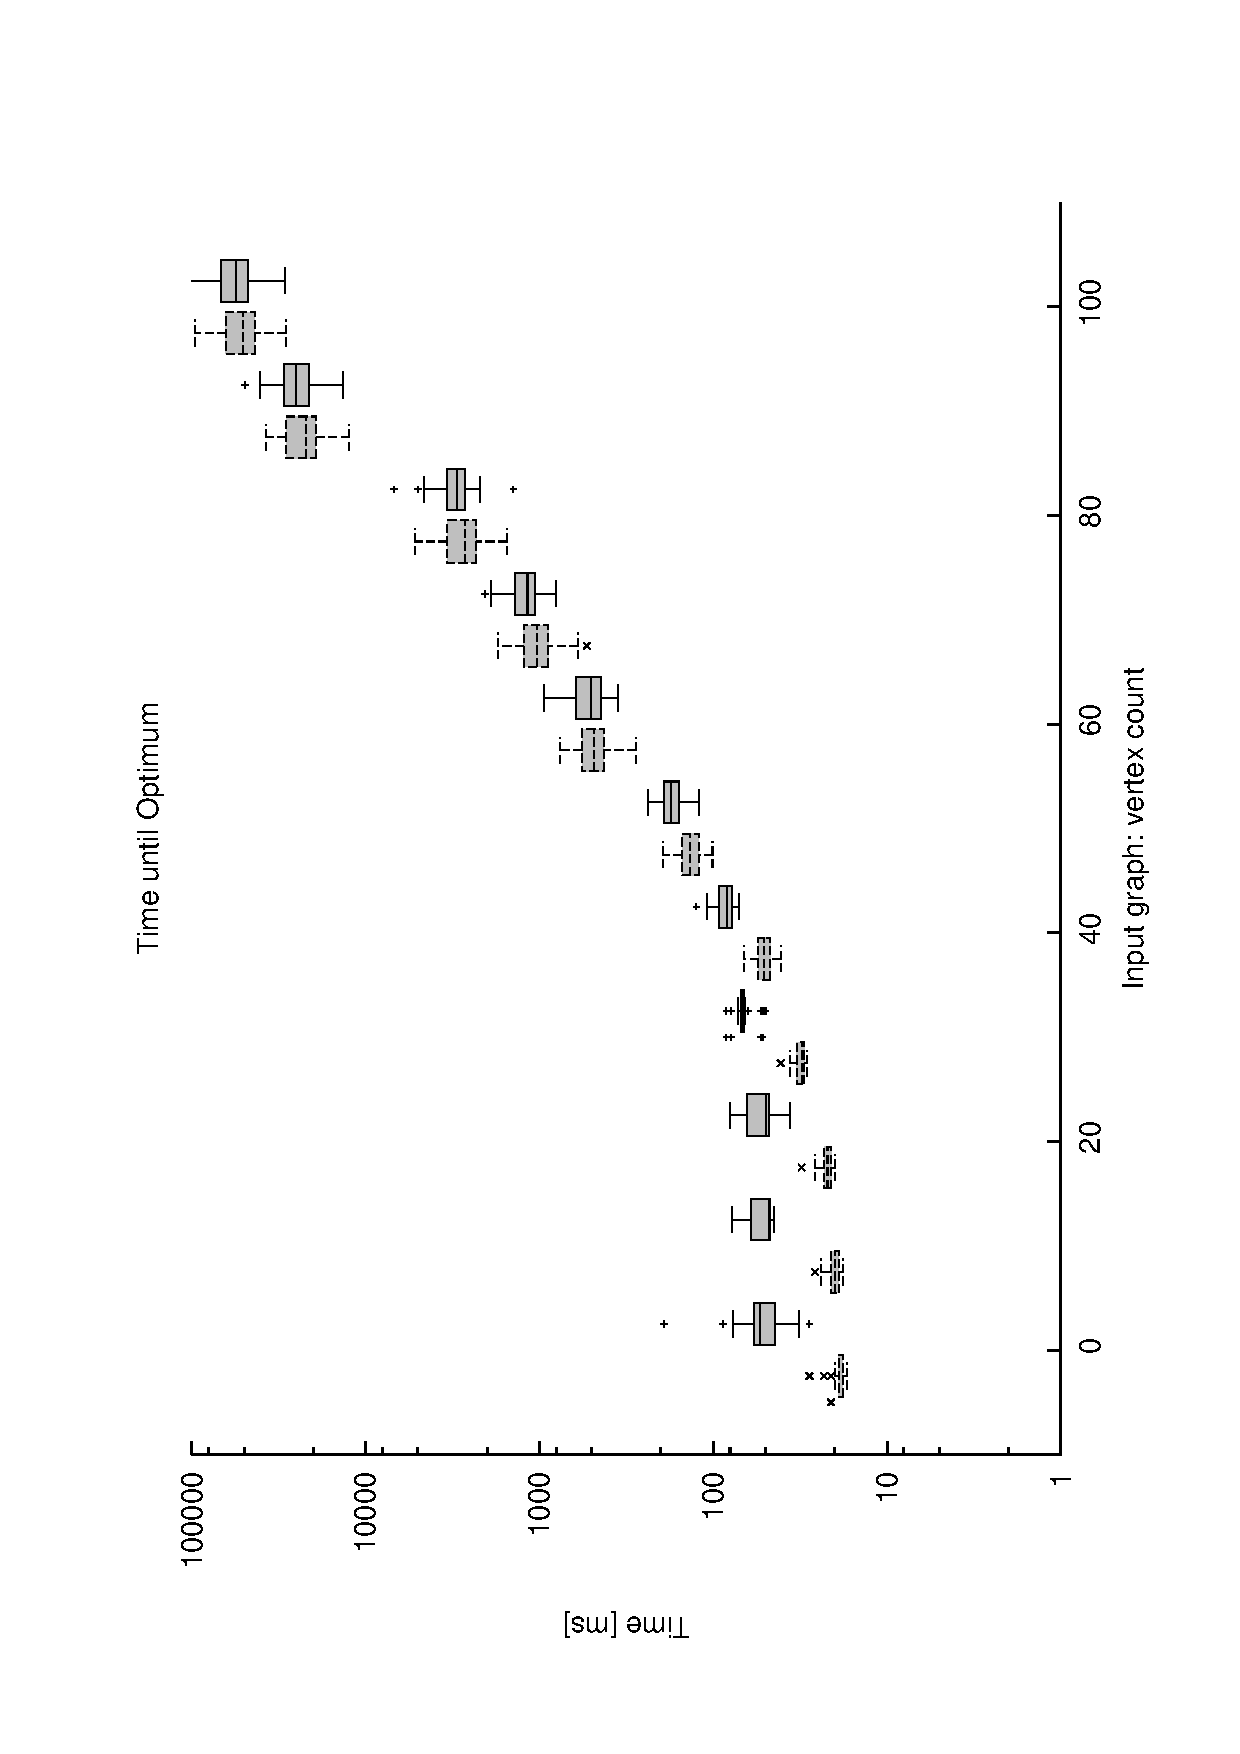
\includegraphics[width=\textwidth]{images/experiments/time-till-optimum}
\end{figure}

TODO interpretation. Graph has its Y axis in log, stress this fact in the text too

TODO mention that these times show we cannot rely on GLPK alone! It just takes too long.

\begin{figure}
  \caption{Timing Summary}
  \label{image-experiment-timing-summary}
  \centering
    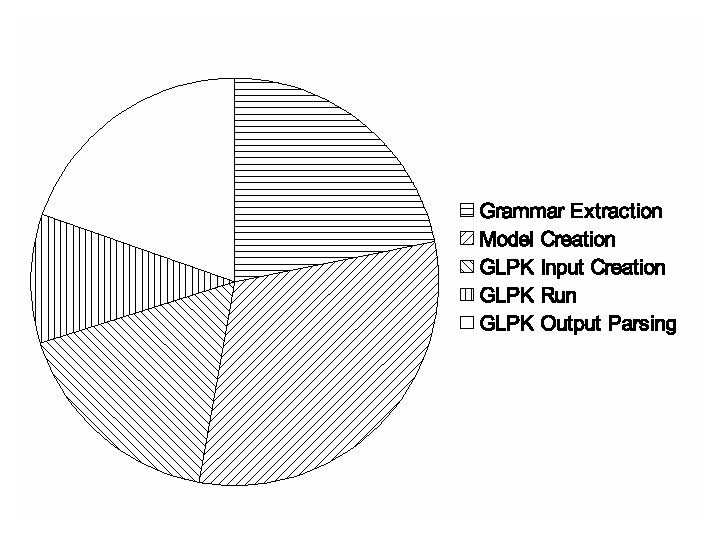
\includegraphics[width=.6\textwidth]{images/experiments/timing-pie}
\end{figure}

TODO interpret

\subsection{\heu{Random} vs. \heu{Fuzzy} vs. \heu{FIDAX}}

%         NB class RandomVsFuzzyVsFidaxStart

Our investigation into various CH will start by comparing \heu{FIDAX} from the original article \cite{fidax} to 2 of our trivial randomized hungry heuristics, \heu{Random} and \heu{Fuzzy}.

\begin{center}
\bigskip
\begin{tabular}{| l | l |}
  \hline
  \hline
  Machine           & Dual Core \\
  Input data set    & all official test data sets \\
  Iterations        & 50 \\
  Pool size         & 10 \\
  $\alpha$, $\beta$ & $1$, $1$ \\
  \hline
\end{tabular}
\bigskip
\end{center}

The experimental set will contain 660 configurations in total: 3 different CHs * 11 official test data sets * 20 iterations. There will be no improvement heuristics. The pool size will be set to 10, even though \heu{FIDAX} cannot not profit from this. Listing for this can be found in \ref{listing-experiment-random-fuzzy-fidax}.

We will be gathering the running time of the CH itself and incumbent qualities (best in the pool) for GnuPlot.

\begin{algorithm}
\caption{\heu{Random} vs. \heu{Fuzzy} vs. \heu{FIDAX} set generation}
\label{listing-experiment-random-fuzzy-fidax}
\begin{algorithmic}
\ENSURE experimental set $ES$
\STATE $ES \gets \emptyset$
\FOR{$i = 1 \to 50$}
	\FOR{$file \in $ official test data}
    \STATE $ES \gets ES \cup \{file, CH = \heu{Random}(pool = 10), IH = \emptyset\} \cup \{file, CH = \heu{Fuzzy}(pool = 10), IH = \emptyset\} \cup \{file, CH = \heu{FIDAX}, IH = \emptyset\}$
  \ENDFOR
\ENDFOR
\RETURN $ES$
\end{algorithmic}
\end{algorithm}

TODO repair outliers in these 2 graphs

\begin{figure}
  \caption{Random vs. Fuzzy vs. FIDAX - Quality}
  \label{image-experiment-random-fuzzy-fidax-quality}
  \centering
    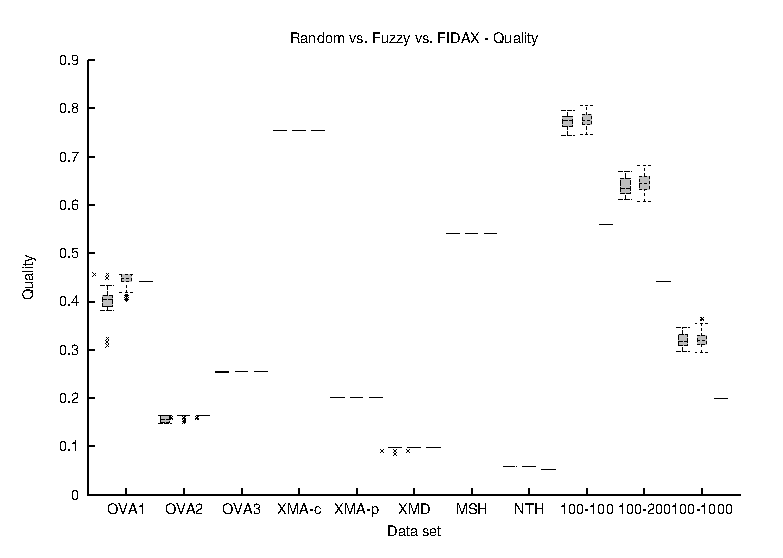
\includegraphics[width=\textwidth]{images/experiments/random-fuzzy-fidax-quality}
\end{figure}

\begin{figure}
  \caption{Random vs. Fuzzy vs. FIDAX - Time}
  \label{image-experiment-random-fuzzy-fidax-time}
  \centering
    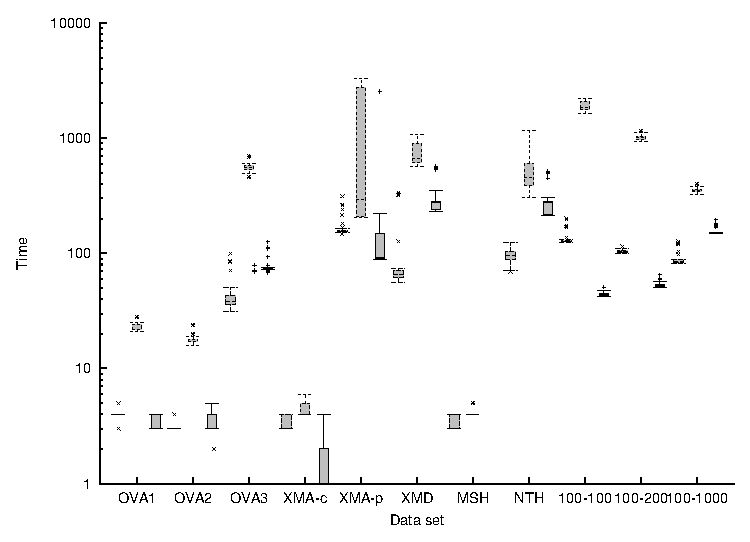
\includegraphics[width=\textwidth]{images/experiments/random-fuzzy-fidax-time}
\end{figure}

TODO interpretation - Fuzzy consistently wins, but takes the longest time by far. Random is better than FIDAX in artificial as well as some real data.

\subsubsection{Improving \heu{FIDAX} with \heu{Hungry}}

%         NB class FidaxWithHungry

There is a minor question to be answered easily: is \heu{FIDAX} ``hungry enough"? Could we improve it using \heu{Hungry} as IH? Let us design a short experiment.

\begin{center}
\bigskip
\begin{tabular}{| l | l |}
  \hline
  \hline
  Machine           & Dual Core \\
  Input data set    & all official test data sets \\
  Iterations        & 1 \\
  Pool size         & 1 \\
  $\alpha$, $\beta$ & $1$, $1$ \\
  \hline
\end{tabular}
\bigskip
\end{center}

We won't be needing pool bigger than one, nor more iterations - both \heu{FIDAX} and \heu{Hungry} are deterministic. We will try all official data sets, first with empty IH, second with \heu{Hungry} as IH. We will gather the qualities in each case and see whether there is any improvement.

The experimental results are summarized in the Table \ref{table-experiments-fidax-and-hungry} and are quite surprising. As trivial a heuristic \heu{Hungry} is, it is still able to improve the ID set found by \heu{FIDAX} by as much as almost 50\% (the last row, \dataset{100-1000}).

Table \ref{table-experiments-fidax-and-hungry-idsets} lists the ID attributes found in both cases for this most extreme input, \dataset{100-1000}. Note that the content of each cell means ``attribute \texttt{attr} in element \texttt{vertexXY} should be marked as ID attribute".

\begin{table}
  \caption{Results of adding \heu{Hungry} after \heu{FIDAX}}
  \bigskip
  \label{table-experiments-fidax-and-hungry}
  \centering
  \begin{tabular}{l | l | l}
    Data set & Quality - \heu{FIDAX} & Quality - \heu{FIDAX} + \heu{Hungry} \\
    \hline
    \dataset{OVA1}     & 0.4411764705882353  & 0.4411764705882353   \\
    \dataset{OVA2}     & 0.16346153846153846 & 0.16346153846153846  \\
    \dataset{OVA3}     & 0.25482414123443264 & \textbf{0.2553715615163541}   \\
    \dataset{XMA-c}    & 0.7546666666666666	 & 0.7546666666666666   \\
    \dataset{XMA-p}    & 0.2019306150568969	 & 0.2019306150568969   \\
    \dataset{XMD}      & 0.09786094165493509 & 0.09786094165493509  \\
    \dataset{MSH}      & 0.5416472778036296	 & 0.5416472778036296   \\
    \dataset{NTH}      & 0.05259709474828076 & \textbf{0.057918595422124436} \\
    \dataset{100-100}  & 0.56	               & \textbf{0.6766666666666669}   \\
    \dataset{100-200}  & 0.44200000000000017 & \textbf{0.5980000000000003}   \\
    \dataset{100-1000} & 0.19952380952380955 & \textbf{0.29619047619047617}  \\
  \end{tabular}
\end{table}

% TODO for some reason \texttt{\textbf{vertex5}} looks only like \texttt{vertex5}
\begin{table}
  \caption{ID sets in \heu{FIDAX} versus \heu{FIDAX} + \heu{Hungry}}
  \bigskip
  \label{table-experiments-fidax-and-hungry-idsets}
  \centering
  \begin{tabular}{l | l}
  \heu{FIDAX} & \heu{FIDAX} + \heu{Hungry} \\
  \hline
                    & \texttt{\textbf{vertex5}}  \\
                    & \texttt{\textbf{vertex26}} \\
  \texttt{vertex30} & \texttt{vertex30} \\
  \texttt{vertex31} & \texttt{vertex31} \\
  \texttt{vertex32} & \texttt{vertex32} \\
  \texttt{vertex34} & \texttt{vertex34} \\
  \texttt{vertex35} & \texttt{vertex35} \\
  \texttt{vertex36} & \texttt{vertex36} \\
  \texttt{vertex37} & \texttt{vertex37} \\
  \texttt{vertex39} & \texttt{vertex39} \\
                    & \texttt{\textbf{vertex60}} \\
                    & \texttt{\textbf{vertex69}} \\
                    & \texttt{\textbf{vertex70}} \\
  \texttt{vertex74} & \texttt{vertex74} \\
  \texttt{vertex75} & \texttt{vertex75} \\
  \texttt{vertex80} & \texttt{vertex80} \\
  \end{tabular}
\end{table}

\subsection{Best standalone CH}

%         NB class BestStandaloneCH

TODO compare all CHs - limit GLPK to 1 second
TODO pool size 10 where applicable

TODO chart for each file: CHs on the X axis, quality Y axis, boxplots

\begin{center}
\bigskip
\begin{tabular}{| l | l |}
  \hline
  \hline
  Machine           & Quad Core \\
  Input data        & all official test data sets \\
  Iterations        & 50 \\
  Pool size         & 10 \\
  $\alpha$, $\beta$ & $1$, $1$ \\
  \hline
\end{tabular}
\bigskip
\end{center}

\begin{algorithm}
\caption{Best Standalone CH set generation}
\label{listing-experiment-best-standalone-ch}
\begin{algorithmic}
\ENSURE experimental set $ES$
\STATE $ES \gets \emptyset$
\FOR{$file \in $ official test data}
	\FOR{$i = 1 \to 50$}
    	\STATE $ES \gets ES \cup \{file, CH = \heu{Random}, IH = \emptyset\}$
    	\STATE $ES \gets ES \cup \{file, CH = \heu{Fuzzy}, IH = \emptyset\}$
    	\STATE $ES \gets ES \cup \{file, CH = \heu{Incremental}, IH = \emptyset\}$
    	\STATE $ES \gets ES \cup \{file, CH = \heu{Removal}, IH = \emptyset\}$
    	\STATE $ES \gets ES \cup \{file, CH = \heu{FIDAX}, IH = \emptyset\}$
    	\STATE $ES \gets ES \cup \{file, CH = \heu{Glpk}(limit = 1), IH = \emptyset\}$
  \ENDFOR
\ENDFOR
\RETURN $ES$
\end{algorithmic}
\end{algorithm}

TODO XMA-c, XMA-p, MSH and NTH are uninteresting - every CH found the optimum every time

\begin{figure}
  \caption{Best Standalone CH}
  \label{image-experiments-best-standalone-ch}
  \centering
  	\subfigure[\dataset{OVA1}]{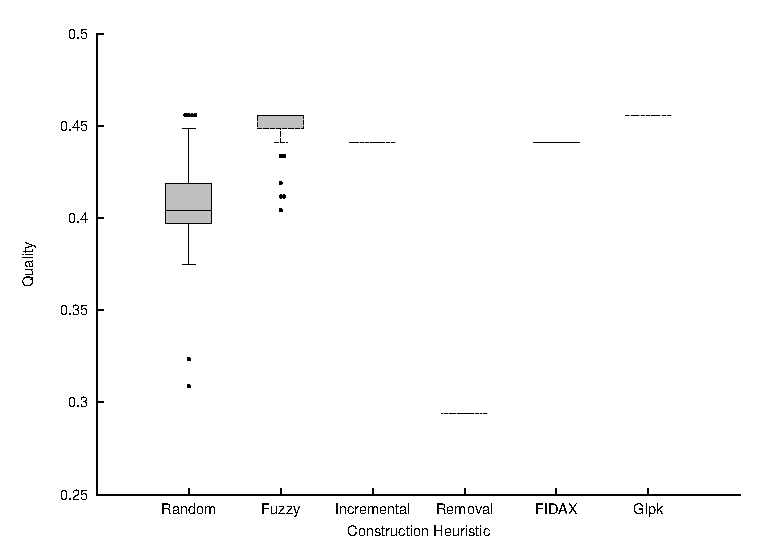
\includegraphics[width=.45\textwidth]{images/experiments/best-ch-OVA1}}
  	\subfigure[\dataset{OVA2}]{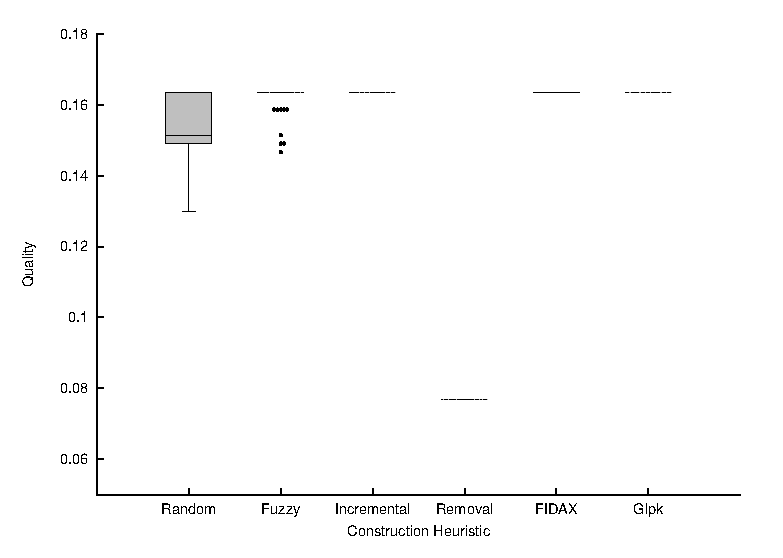
\includegraphics[width=.45\textwidth]{images/experiments/best-ch-OVA2}}
  	\subfigure[\dataset{OVA3}]{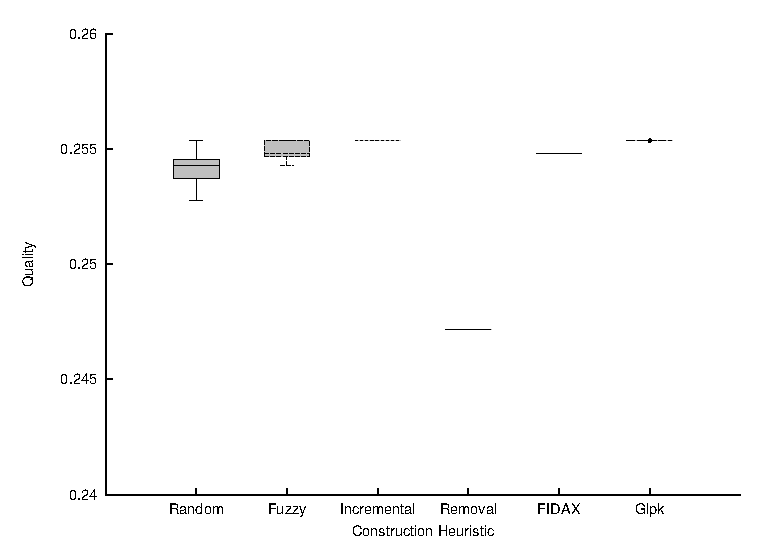
\includegraphics[width=.45\textwidth]{images/experiments/best-ch-OVA3}}
  	\subfigure[\dataset{XMD}]{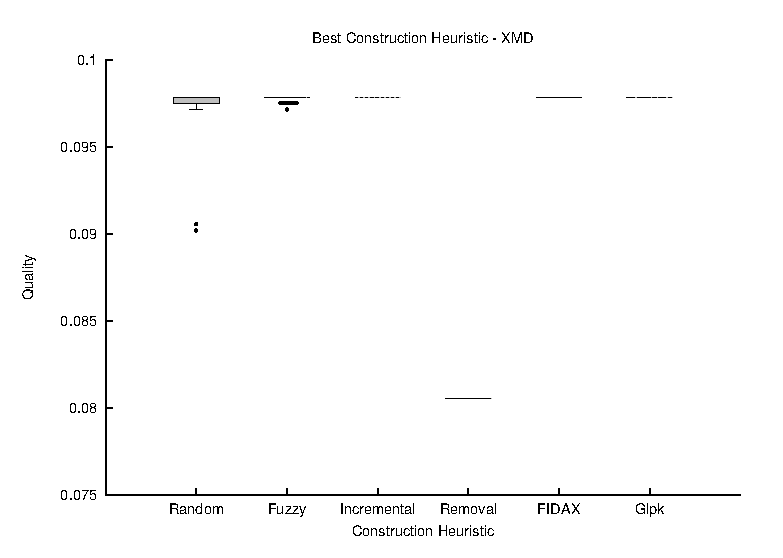
\includegraphics[width=.45\textwidth]{images/experiments/best-ch-XMD}}
   	\subfigure[\dataset{100-100}]{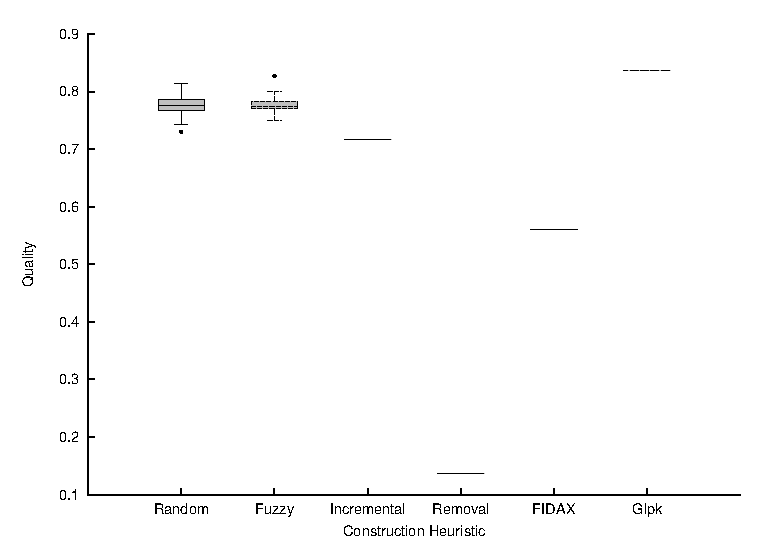
\includegraphics[width=.45\textwidth]{images/experiments/best-ch-100-100}}
  	\subfigure[\dataset{100-200}]{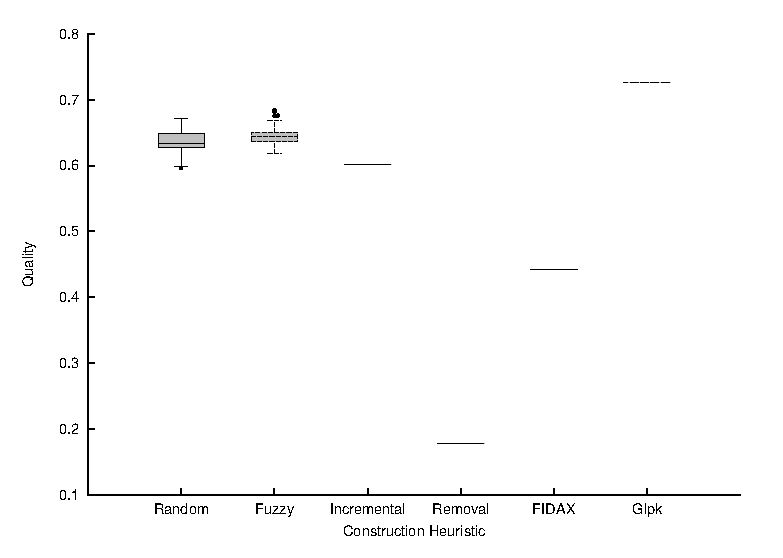
\includegraphics[width=.45\textwidth]{images/experiments/best-ch-100-200}}
  	\subfigure[\dataset{100-1000}]{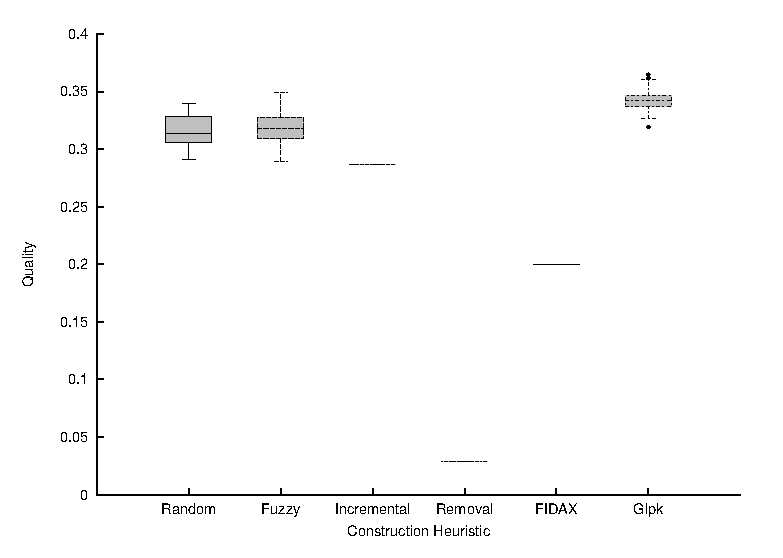
\includegraphics[width=.45\textwidth]{images/experiments/best-ch-100-1000}}
\end{figure}

TODO interpretation - GLPK wins all the time, takes 1 second, which is OK.

\subsection{Best IH for Glpk}

%         NB class BestIHForGlpk

TODO with the best construction heuristic (Glpk), which IH is the best? Note that this needn't be the best combination!

TODO we will ignore RandomRemove and RemoveWorst, they cannot help us

TODO we will be using only a few sets where we can observe improvement

\begin{center}
\bigskip
\begin{tabular}{| l | l |}
  \hline
  \hline
  Machine           & Dual Core \\
  Input data        & \dataset{80-30}, \dataset{90-405}, \dataset{100-500}, \\
                    & \dataset{100-100}, \dataset{100-200}, \dataset{100-1000} \\
  Iterations        & 50 \\
  Pool size         & 10 \\
  $\alpha$, $\beta$ & $1$, $1$ \\
  \hline
\end{tabular}
\bigskip
\end{center}

\begin{algorithm}
\caption{Best IH for \heu{Glpk} set generation}
\label{listing-experiment-best-ih-for-glpk}
\begin{algorithmic}
\ENSURE experimental set $ES$
\STATE $ES \gets \emptyset$
\FOR{$file \in \{\dataset{80-30}, \dataset{90-405}, \dataset{100-500}, \dataset{100-100}, \dataset{100-200}, \dataset{100-1000}\}$}
	\FOR{$i = 1 \to 50$}
    	\STATE $ES \gets ES \cup \{file, CH = \heu{Glpk}(limit = 1), IH = \heu{Crossover}(ratio = 0.1, limit = 1)\}$
    	\STATE $ES \gets ES \cup \{file, CH = \heu{Glpk}(limit = 1), IH = \heu{Hungry}\}$
    	\STATE $ES \gets ES \cup \{file, CH = \heu{Glpk}(limit = 1), IH = \heu{Local Branching}(ratio = 0.1, limit = 1)\}$
    	\STATE $ES \gets ES \cup \{file, CH = \heu{Glpk}(limit = 1), IH = \heu{Mutation}(ratio = 0.1, limit = 1)\}$
  \ENDFOR
\ENDFOR
\RETURN $ES$
\end{algorithmic}
\end{algorithm}

\begin{table}
  \caption{Best IH for \heu{Glpk}}
  \bigskip
  \label{table-experiments-best-ih-for-glpk}
  \centering
  \begin{tabular}{l || l | l || l | l}
    Data set & \heu{Hungry} & \heu{Hungry} & \heu{Crossover} & \heu{Crossover} \\
     & improvement & improvement & improvement & improvement \\
     & avg & stdev & avg & stdev \\
    \hline
    \dataset{80-320} & 0.00017 & 0.00118 & 0.00017 & 0.00118 \\
    \dataset{90-405} & 0.00502 & 0.00618 & 0.00033 & 0.00165 \\
    \dataset{100-500} & 0.00664 & 0.00667 & 0.00016 & 0.00081 \\
    \hline
    \dataset{100-100} & 0.00000 & 0.00000 & 0.00000 & 0.00000 \\
    \dataset{100-200} & 0.00000 & 0.00000 & 0.00000 & 0.00000 \\
    \dataset{100-1000} & 0.01630 & 0.01294 & 0.00180 & 0.00506 \\
  \end{tabular}    
	% TODO separate somehow
  \begin{tabular}{l || l | l || l | l}
    Data set & \heu{LB} & \heu{LB} & \heu{Mutation} & \heu{Mutation} \\
     & improvement & improvement & improvement & improvement \\
     & avg & stdev & avg & stdev \\
    \hline
    \dataset{80-320} & \textbf{0.00072} & 0.00223 & 0.00064 & 0.00218 \\
    \dataset{90-405} & 0.00698 & 0.00616 & \textbf{0.00851} & 0.00659 \\
    \dataset{100-500} & 0.00796 & 0.00797 & \textbf{0.00964} & 0.00804 \\
    \hline
    \dataset{100-100} & 0.00000 & 0.00000 & 0.00000 & 0.00000 \\
    \dataset{100-200} & 0.00000 & 0.00000 & 0.00000 & 0.00000 \\
    \dataset{100-1000} & 0.01710 & 0.01188 & \textbf{0.02337} & 0.01558 \\
  \end{tabular}
\end{table}

TODO interpretation: \heu{Mutation} wins.

\subsubsection{\heu{Random} as CH}

%         NB class CHForMutation

TODO with \heu{Mutation} from the previous step, how about using Random as CH? Do we get an improvement?

\begin{center}
\bigskip
\begin{tabular}{| l | l |}
  \hline
  \hline
  Machine           & Dual Core \\
  Input data        & \dataset{80-30}, \dataset{90-405}, \dataset{100-500}, \\
                    & \dataset{100-100}, \dataset{100-200}, \dataset{100-1000} \\
  Iterations        & 50 \\
  Pool size         & 10 \\
  $\alpha$, $\beta$ & $1$, $1$ \\
  \hline
\end{tabular}
\bigskip
\end{center}

\begin{algorithm}
\caption{\heu{Random} as CH set generation}
\label{listing-experiment-ch-for-mutation}
\begin{algorithmic}
\ENSURE experimental set $ES$
\STATE $ES \gets \emptyset$
\FOR{$file \in \{\dataset{80-30}, \dataset{90-405}, \dataset{100-500}, \dataset{100-100}, \dataset{100-200}, \dataset{100-1000}\}$}
	\FOR{$i = 1 \to 50$}
    	\STATE $ES \gets ES \cup \{file, CH = \heu{Random}, IH = \heu{Mutation}(ratio = 0.1, limit = 1)\}$
    	\STATE $ES \gets ES \cup \{file, CH = \heu{Glpk}(limit = 1), IH = \heu{Mutation}(ratio = 0.1, limit = 1)\}$
  \ENDFOR
\ENDFOR
\RETURN $ES$
\end{algorithmic}
\end{algorithm}

\begin{figure}
  \caption{CH for \heu{Mutation}}
  \label{image-experiment-ch-for-mutation}
  \centering
    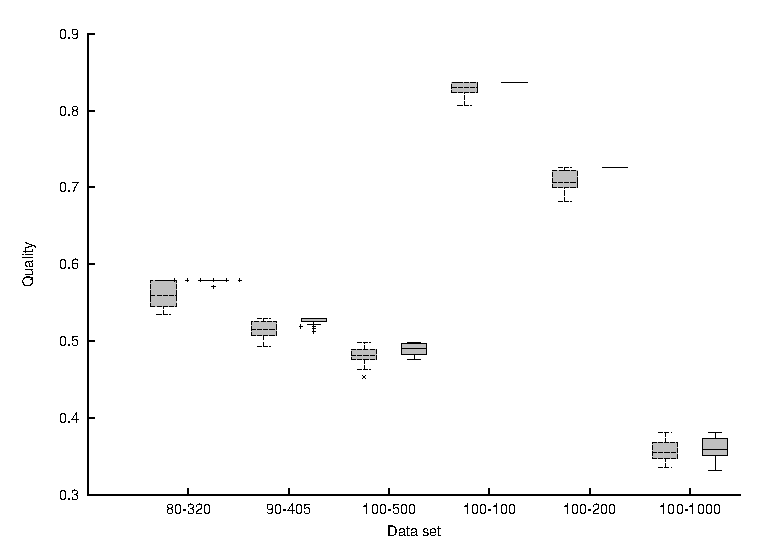
\includegraphics[width=\textwidth]{images/experiments/ch-for-mutation}
\end{figure}

TODO odd are random, even are Glpk

TODO interpretation - Glpk as CH takes always one second, with simpler inputs almost always finds the optimum (thus the capping), with more complex is Random not that bad in the end

\subsection{Various $\alpha$, $\beta$}

TODO remind what these parameters mean

TODO summary table

TODO pseudocode

TODO results - perhaps use the images from graph representation, highlight various sets?

TODO interpretation

\subsection{Various Ratios in IHs}

TODO

TODO summary table

TODO pseudocode

TODO results

TODO interpretation

\subsection{Ignoring text data}

%         NB class IgnoreTextData

TODO can we improve performance on huge data by ignoring textual content? Check for building as well as actual heu times.

\begin{center}
\bigskip
\begin{tabular}{| l | l |}
  \hline
  \hline
  Machine           & Dual Core \\
  Input data        & \dataset{XMA-p} \\
  Iterations        & 50 \\
  Pool size         & TODO \\
  $\alpha$, $\beta$ & $1$, $1$ \\
  \hline
\end{tabular}
\bigskip
\end{center}

TODO pseudocode

\begin{figure}
  \caption{Ignoring Text Data}
  \label{image-experiment-ignore-text-data}
  \centering
    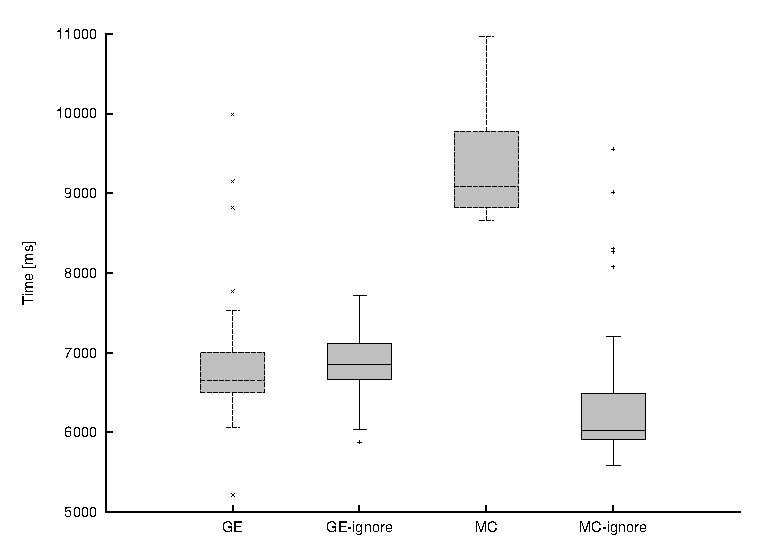
\includegraphics[width=\textwidth]{images/experiments/ignore-text-data}
\end{figure}

TODO interpretation

\subsection{Chaining the IHs}

TODO finally we got to the most interesting part, unfortunately this is basically guesswork and intuition.

\subsection{Algorithms for various data characteristics}

TODO

\section{The "Best" Algorithm}

TODO we have asked a lot of questions and got the answers, now is the time to summarize, to find some "wisdom".

First of all: if we have the time, it is best to just let the GLPK run.
We will find the optimum in this way.
And for many purposes, this is just fine - we need to infer something about the schema, we do it only once, so it doesn't matter that much how long it takes.

Second: if we don't have enough time, we should do XYZ but it might depend on the characteristics of the data.
For realistic (looks like THIS in graph representation) it is best to do A B C.
Whereas, for artificial data (having IJK as their representation) it is best to just do 1 2 3.


\chapter{Future work}

TODO

\begin{itemize}
  \item extension to more documents at once
  \item more heuristics and their chaining
  \item ACO, genetic, ...
  \item user-friendly experimental interface (choose and setup experiments on the fly in GUI)
  \item jInfer is opensource, thus easy to extend!
\end{itemize}


\chapwithtoc{Conclusion}

From all the integrity constraints in XML we chose the \texttt{ID}/\.\texttt{IDREF}/\.\texttt{IDREFS} attributes and decided to improve upon the search for them. We discussed the approach from \cite{fidax} and the equivalence of ID set search and maximum weighted independent set. Based on this article we introduced the MIP approach and demonstrated how to find the optimal ID set using external GLPK solver in the environment of jInfer framework.\\

However, this approach took too long for some inputs, so we introduced a~whole range of construction as well as improvement heuristics. We combined these algorithms to create a metaheuristic and performed a number of experiments to understand its behavior. Finally we selected a promising metaheuristic strategy and tuned its parameters to find very good ID sets while maintaining low running times.\\

To the best of our knowledge, at the time of writing this work is our approach to finding \texttt{ID} attributes the best one known.\\

The wisdom found in the experiments in this work might be the following. While it is important to be able to write a heuristic algorithm tailored to the specific problem being solved, such as the authors of \cite{fidax} did, it should be noted that sometimes it is better to solve a more general problem. In~this case the transformation to MIP formulation and using a dedicated solver proved to~produce better results in shorter time.

%%% Seznam použité literatury
\newpage
\nocite{*}
\bibliographystyle{alpha}
\bibliography{literature}

\listoffigures
\addcontentsline{toc}{chapter}{List of Figures}

\listofalgorithms
\addcontentsline{toc}{chapter}{List of Algorithms}

%%% Tabulky v diplomové práci, existují-li.
%\chapwithtoc{List of Tables}
\listoftables
\addcontentsline{toc}{chapter}{List of Tables}

%%% Použité zkratky v diplomové práci, existují-li, včetně jejich vysvětlení.

\printnomenclature[2cm]
\addcontentsline{toc}{chapter}{List of Abbreviations}

%%% Přílohy k diplomové práci, existují-li (různé dodatky jako výpisy programů,
%%% diagramy apod.). Každá příloha musí být alespoň jednou odkazována z vlastního
%%% textu práce. Přílohy se číslují.

\appendix

\openright
\addcontentsline{toc}{chapter}{Appendices}

\chapter{jInfer}
\label{appendix-jInfer}

This appendix will try to describe shortly yet comprehensively \textbf{jInfer} - the Java framework for XML schema inference. Please see project web \cite{jinferweb} for complete information, documentation and download options.

jInfer was developed between 2009 and 2011 at Charles University in Prague as a Software Project by team consisting of Michal Klempa, Mario Mikula, Ro\-bert Sme\-ta\-na, Michal Svirec and Matej Vitasek. The main idea was to create a structure in which all aspects of XML schema inference can be easily implemented and evaluated. The goal was achieved: the SW project was successfuly defended when jInfer was inferring DTD and XSD schemas based on XML documents, old DTD and XSD schemas and XPath queries. Since then, Michal Klempa has successfuly defended his own thesis improving on the grammar simplification process (see below), Michal Svirec has extended the framework with capabilities to detect and repair functional dependencies violation and defended his thesis as well. This thesis is the third based on this framework, and Mario Mikula's is on its way, too.

To the best of our knowledge, at the time of writing this thesis is jInfer the only public, open source and actually working solution for XML schema inference-related tasks.

At heart of jInfer inference process is a modular system provided by NetBeans Platform allowing to define services (interfaces), implement them in any number of ways and then let the user choose which implementation to use. Most importantly, the whole process consists of 3 consecutive steps (see \ref{image-inference-process}), responsibility of 3 different services - interchangeable modules.

\begin{figure}
  \caption{Inference process in jInfer}
  \label{image-inference-process}
  \centering
    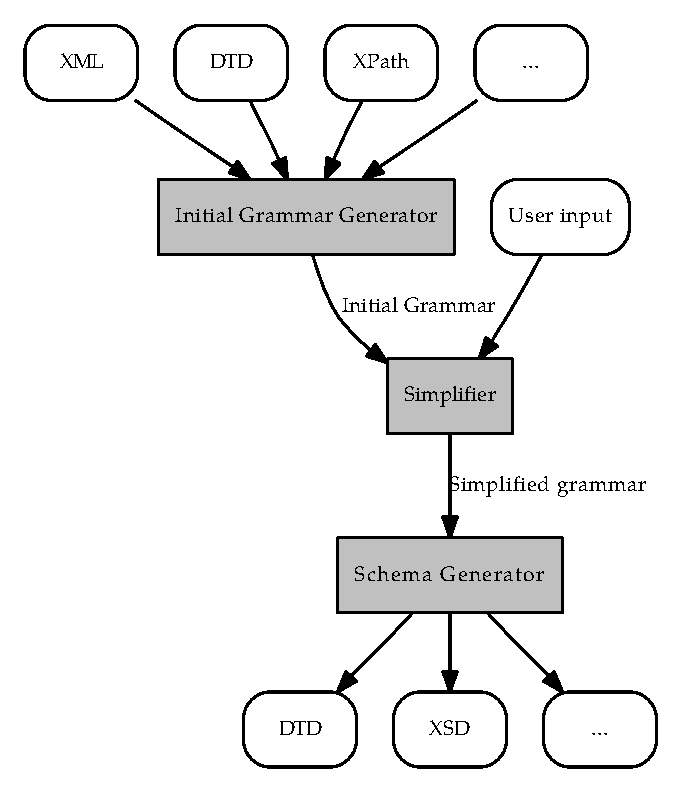
\includegraphics[width=0.5\textwidth]{images/inference-process}
\end{figure}

The responsibility of the first module, the \jmodule{Initial Grammar Generator}, is to parse all input files (documents, schemas and queries) and create a so-called \textit{initial grammar} (IG, TODO nomenclature). This is the representation in which will the structure live until it is used to create the final product - the schema. As the name suggests, IG is a grammar - an \textit{extended context-free grammar}, to be more precise (see \cite{extendedcfg}). As such, its left hand side is an element, its right hand side is a regular expression representing its content model. (TODO picture?) IG is used to create the AM model used in this thesis, too. jInfer contains one such module, the \jmodule{BasicIGG}, which is described in detail in \cite{basiciggdoc}.

After leaving the \jmodule{Initial Grammar Generator}, the IG needs to be made more general, shortened, \textit{simplified}. This is the responsibility of an aptly named module, the \jmodule{Simplifier}. To get the full idea about how this can be done it would be probably best to read Michal Klempa's thesis (TODO link), which describes this in great detail. Whatever happens, there is simplified grammar on the exit of \jmodule{Simplifier}, ready to be processed by...

The last module, \jmodule{Schema Generator} takes the simplified grammar and creates the resulting schema from it. This process is not too interesting, but anyone wishing to find out all about it is invited to read the documentation to the two \jmodule{Schema Generator}s bundled with jInfer - the BasicDTD and BasicXSD modules.

\chapter{\jmodule{IDSetSearch}}
\label{appendix-iss}

This appendix will shortly describe the \jmodule{IDSetSearch} jInfer module. As the name suggests, its main purpose is to find ID and IDREF sets and provide attribute statistics in general for grammars originating from any stage of XML schema inference. Virtually every piece of code that was added to jInfer in the course of creating this thesis is contained in this module.\\

From jInfer's point of view, this module resides in codebase \texttt{cz.\.cuni.\.mff.\.ksi.\.jinfer.\.iss} and is a service provider for \texttt{cz.\.cuni.\.mff.\.ksi.\.jinfer.\.base.\.inter\.faces.\.ID\.Set\.Search} interface. Invoking the \texttt{showIDSetPanel()} method displays a fully-featured window containing all the relevant attribute statistics as well as possibility to find the ID and IDREF sets for a specified grammar.\\

Most important packages in \jmodule{IDSetSearch} are the following.

\begin{itemize}
	\item \texttt{objects}, containing the object representation of attribute mappings and AM model.
	\item \texttt{heuristics.construction}, containing all the CHs hidden behind the \texttt{Con\-struc\-tion\-Heu\-ris\-tic} interface, with sub-packages \texttt{fidax} containing the whole implementation of FIDAX heuristic % TODO link
	and \texttt{glpk} containing the whole interface to an external GLPK solver. % TODO link
	\item \texttt{heuristics.improvement}, containing all the IH hidden behind the \texttt{Im\-prove\-ment\-Heu\-ris\-tic} interface.
	\item \texttt{experiments}, containing everything related to experimenting with these heuristics.
\end{itemize}

\texttt{Experiment} is a class representing a single experiment with specified input data (encapsulated in \texttt{Test\-Data} interface), settings (encapsulated in \texttt{Ex\-pe\-ri\-ment\-Pa\-ra\-me\-ters}) and a metaheuristic as defined in TODO link. Its method \texttt{run()} will launch the metaheuristic, first executing the construction heuristic and then running the specified improvement heuristics in a loop until termination criteria defined in an implementation of \texttt{Ter\-mi\-na\-tion\-Cri\-ter\-ion} are met. The quality of a single ID set is measured by an instance of \texttt{Quality\-Measurement}. After the experiment finishes, it invokes the \texttt{notify\-Finished()} method.\\

However, experiments are almost never run alone. For the purpose of running a whole experimental set there is the \texttt{Experiment\-Set} interface and its abstract implementation \texttt{Abstract\-Experiment\-Set}. Its descendants need only to provide a list of \texttt{Experiment\-Parameter}s and looping as well as data collection will be handled for them.

\section{How to Create a New Heuristic}

Decide whether it should be a CH or IH and create a class implementing \texttt{Con\-struc\-tion\-Heu\-ris\-tic} or \texttt{Im\-prove\-ment\-Heu\-ris\-tic}, respectively. In each case implement all the \texttt{get*Name()} methods inherited from \texttt{Named\-Module} and then the most important \texttt{start()} method.

In this method use the provided \texttt{Experiment} instance (and \texttt{List<IdSet> feasiblePool} in case of IH) to create a pool of feasible solutions and in the end return it by invoking the \texttt{finished()} method of the provided \texttt{Heuristic\-Callback} parameter.

\section{How to Create a New Experimental Set}

Subclass the \texttt{Abstract\-Experiment\-Set} class, override \texttt{get\-Name()} to provide the name of this set and finally override \texttt{get\-Experiments()} to return the list of \texttt{Experiment\-Parameters} that will constitute this sit.

It is possible to optionaly override any of the following methods: \texttt{notify\-Start()}, \texttt{notify\-Finished()} and \texttt{notify\-Finished\-All()}. They will be invoked before running the first experiment, after each experiment run and after all experiments finished, respectively. Note that \texttt{notify\-Finished()} already contains logic to output some information regarding the currently finished experiment to a file, but it can be safely overriden without a need to call \texttt{super.\.notify\-Finished()}.

\chapter{Experimental Trace}
\label{appendix-trace}

Following is a trace logged from a sample experiment run. It shows all the relevant information related to this instance, any and every piece of information we might be interested in.

To save space, 2-column layout is used. Commentary on the particulars follows right after its end.

\begin{multicols}{2}
\begin{scriptsize}
\begin{verbatim}
CPU info
  Intel(R) Core(TM)2 Quad CPU Q9550 @ 2.83GHz
  Cores: 4
  Clock speed: 2983 MHz
Memory info
  Size: 8192 MB
OS info
  Name: Windows 7
  Version: 6.1
  Architecture: amd64
Java info
  Version: 1.6.0_26
  VM: Java HotSpot(TM) 64-Bit Server VM
GLPK info
  GLPSOL: GLPK LP/MIP Solver 4.34

Configuration:
File name: graph.xml (101599 b)
  Graph representation: 82 vertices, 1101 edges
alpha: 1.0, beta: 1.0

Results:
Total time spent: 7754 ms
Final quality: 0.19951219512195123 (10 AMs)
Highest quality: 0.23463414634146343 (12 AMs)
Construction phase:
  Algorithm: Random
    Time taken: 248 ms / Time since start: 248 ms
    Pool size: 10
    Quality: 0.19975609756097568 (11 AMs)
Improvement phase:
  pass #1:
  Algorithm: RandomRemove, ratio = 0.2
    Time taken: 0 ms / Time since start: 841 ms
    Pool size: 10
    Quality: 0.15878048780487808 (9 AMs)
  pass #2:
  Algorithm: Mutation, ratio = 0.1, limit = 1 s
    Time taken: 1512 ms / Time since start: 2710 ms
    Pool size: 11
    Quality: 0.21975609756097558 (11 AMs)

  <... 7 more passes removed ...>

  pass #10:
  Algorithm: Remove Worst
    Time taken: 80 ms / Time since start: 7676 ms
    Pool size: 12
    Quality: 0.19951219512195123 (10 AMs)
Termination reason: Maximum iterations exceeded.

Time,Quality,AMs
248,0.19975609756097568,11
841,0.15878048780487808,9
2710,0.21975609756097558,11
2927,0.1890243902439024,9
4421,0.23463414634146343,12
4703,0.23463414634146343,12
4896,0.1960975609756098,10
5793,0.23463414634146337,12
5972,0.19951219512195123,10
7433,0.19951219512195123,10
7676,0.19951219512195123,10

ID
Element,Attribute,Weight
vertex0,attr,0.024146341463414635
vertex2,attr,0.01975609756097561
vertex33,attr,0.016829268292682928
vertex34,attr,0.02219512195121951
vertex4,attr,0.022682926829268292
vertex41,attr,0.014878048780487804
vertex7,attr,0.02170731707317073
vertex70,attr,0.018780487804878048
vertex76,attr,0.01780487804878049
vertex8,attr,0.02170731707317073
vertex80,attr,0.01780487804878049
vertex97,attr,0.016341463414634147

IDREF
Element,Attribute
\end{verbatim}
\end{scriptsize}
\end{multicols}

The first section deals with system information. Please note that some of these characteristics cannot be easily obtained programmatically and are thus stored in the source code as constants.\\
To obtain GLPK information, the program parses the first line of standard output produced by running \code{glpsol -v}. It tries to guess whether it's the Cygwin version by looking at the path to the binary.

The second section states the input file along with its size and graph representation (Section \ref{section-experiments-data}). Alpha and beta parameters for this instance belong here too.

\begin{footnotesize}
\begin{verbatim}
Configuration:
File name: graph.xml (101599 b)
  Graph representation: 82 vertices, 1101 edges
alpha: 1.0, beta: 1.0
\end{verbatim}
\end{footnotesize}

Results section opens stating the most important information first: how long did the experiment run and what was the highest and final quality (these two are potentially different). Numbers of attribute mappings in the best and final solution respectively are stated as well.

\begin{footnotesize}
\begin{verbatim}
Total time spent: 7754 ms
Final quality: 0.19951219512195123 (10 AMs)
Highest quality: 0.23463414634146343 (12 AMs)
\end{verbatim}
\end{footnotesize}

Construction phase results go next. Among reported information are the full identification of the heuristic (possibly along with its parameters), time taken, size of the pool created and the quality of the incumbent solution (again, with the number of its AMs).

\begin{footnotesize}
\begin{verbatim}
Algorithm: Random
  Time taken: 248 ms / Time since start: 248 ms
  Pool size: 10
  Quality: 0.19975609756097568 (11 AMs)
\end{verbatim}
\end{footnotesize}

Now for each of the improvement phases there is one section in output log. Information presented here has the same structure as with the construction phase. Please note that the \code{Pool size} is always measured \textit{after} the improvement run.

\begin{footnotesize}
\begin{verbatim}
Algorithm: Mutation, ratio = 0.1, limit = 1 s
  Time taken: 1512 ms / Time since start: 2710 ms
  Pool size: 11
  Quality: 0.21975609756097558 (11 AMs)
\end{verbatim}
\end{footnotesize}

After the last improvement phase, the reason why the metaheuristic terminated is stated. Possible causes are exceeding the maximum time available, maximum iterations or reaching the known optimum for this file and alpha / beta settings.
\\

To be able to reconstruct the progress of the metaheuristic, the next section contains CSV \nomenclature{CSV}{Comma Separated Values} formatted data for each iteration. Each row contains the time in milliseconds, quality of the incumbent solution and the number of its AMs.

\begin{footnotesize}
\begin{verbatim}
Time,Quality,AMs
...
841,0.15878048780487808,9
2710,0.21975609756097558,11
...
\end{verbatim}
\end{footnotesize}

And finally, it is important to know what is the ID/IDREF set recommended by this experiment run - the reason why we do all this! Thus the log is concluded by a CSV formatted list of element - attribute name pairs to be included in the ID and IDREF set, respectively.

\begin{footnotesize}
\begin{verbatim}
Element,Attribute,Weight
vertex0,attr,0.024146341463414635
...
\end{verbatim}
\end{footnotesize}

Note that in this example trace there were no \texttt{IDREF} AMs found. \qed

\flushright
$\square$

\end{document}
